
\documentclass[12pt,a4paper]{report}

% Packages
\usepackage[a4paper, margin=1in]{geometry}
\usepackage{graphicx}
\usepackage{amsmath}
\usepackage{amssymb}
\usepackage{booktabs}
\usepackage{array}
\usepackage{tabularx}
\usepackage{float}
\usepackage{fancyhdr}
\usepackage[hidelinks]{hyperref}
\usepackage{xcolor}
\usepackage{setspace}
\usepackage{enumitem}
\usepackage{caption}

\captionsetup{
    labelfont=bf,
    justification=raggedright,
    singlelinecheck=false,
    format=plain
}
\usepackage{subcaption}
\usepackage{multirow}
\usepackage{colortbl}
\usepackage{longtable}
\setlength{\LTleft}{\fill}
\setlength{\LTright}{\fill}
\usepackage{titlesec}
\usepackage{titletoc}
\usepackage{lastpage}
\usepackage{makecell}
\usepackage{etoolbox}
\usepackage{needspace}

\numberwithin{figure}{chapter}
% Shared table layout and spacing
\setlength{\tabcolsep}{6pt}
\renewcommand{\arraystretch}{1.12}
\setlength{\LTpre}{0pt}
\setlength{\LTpost}{6pt}
\setlength{\arrayrulewidth}{0.5pt}
\setlength{\extrarowheight}{0.6pt}
\setlength{\footskip}{42pt}
\setlength{\headheight}{18pt}

% Prevent tables from overflowing past the page bottom:
% if fewer than 5 baseline-skips remain, break to the next page first.
\BeforeBeginEnvironment{table}{\needspace{5\baselineskip}}
\BeforeBeginEnvironment{longtable}{\Needspace{5\baselineskip}}

\definecolor{osdagGreen}{HTML}{91B014}

\fancypagestyle{main}{
  \fancyhf{}
  \fancyhead[L]{Synthetic Bridge Integration Test $|$ SYNTHETIC-001}
  \fancyhead[R]{2026-11-20 $|$ Synthetic Report Validation}
  \fancyfoot[L]{Prepared with OsdagBridge}
  \fancyfoot[R]{Page \thepage\ of \pageref{LastPage}}
  \renewcommand{\headrule}{\color{osdagGreen}\hrule width\headwidth height 1pt \vspace{2pt}}
  \renewcommand{\footrule}{%
    \ifbool{hasSDonPage}{%
      \vspace{2pt}%
      \hbox to \headwidth{\textcolor{black}{\footnotesize\textit{* Software default value}}\hfil}%
      \vspace{4pt}%
    }{%
      \vspace{2pt}%
    }%
    \color{osdagGreen}\hrule width\headwidth height 1pt \vspace{6pt}%
  }
}
\fancypagestyle{plain}{
  \fancyhf{}
  \fancyhead[L]{Synthetic Bridge Integration Test $|$ SYNTHETIC-001}
  \fancyhead[R]{2026-11-20 $|$ Synthetic Report Validation}
  \fancyfoot[L]{Prepared with OsdagBridge}
  \fancyfoot[R]{Page \thepage\ of \pageref{LastPage}}
  \renewcommand{\headrule}{\color{osdagGreen}\hrule width\headwidth height 1pt \vspace{2pt}}
  \renewcommand{\footrule}{%
    \ifbool{hasSDonPage}{%
      \vspace{2pt}%
      \hbox to \headwidth{\textcolor{black}{\footnotesize\textit{* Software default value}}\hfil}%
      \vspace{4pt}%
    }{%
      \vspace{2pt}%
    }%
    \color{osdagGreen}\hrule width\headwidth height 1pt \vspace{6pt}%
  }
}
\fancypagestyle{firstpage}{
  \fancyhf{}
  \renewcommand{\headrulewidth}{0pt}
  \fancyfoot[L]{Prepared with OsdagBridge}
  \fancyfoot[R]{Page \thepage\ of \pageref{LastPage}}
  \renewcommand{\footrule}{\vspace{-8pt}\color{osdagGreen}\hrule width\headwidth height 1pt \vspace{6pt}}
}
\pagestyle{main}
\setstretch{1.15}

% Custom Commands
\newcommand{\placeholder}[1]{\textit{\textless #1\textgreater}}
\newcommand{\todo}[1]{\colorbox{yellow}{TODO: #1}}
\newcolumntype{L}[1]{>{\raggedright\arraybackslash}p{#1}}
\newcolumntype{C}[1]{>{\centering\arraybackslash}p{#1}}
\newcolumntype{R}[1]{>{\raggedleft\arraybackslash}p{#1}}

% Software-default asterisk
\newcommand{\sdstar}{\textsuperscript{*}}
\newbool{hasSDonPage}
\boolfalse{hasSDonPage}
\newcommand{\markSD}{\global\booltrue{hasSDonPage}}
\renewcommand{\sdstar}{\textsuperscript{*}\markSD{}}
\AddToHook{shipout/before}{\global\boolfalse{hasSDonPage}}

\title{\Large\textbf{OsdagBridge} \\ \normalsize Open Source Software for Steel Girder Bridge Design \\ \vspace{2cm} \large Design Report}
\author{}
\date{}

\begin{document}


\begin{titlepage}
\thispagestyle{firstpage}
\centering
\vspace*{1.5cm}
\noindent
\begin{minipage}[c]{0.6\textwidth}
\raggedright

\includegraphics[width=\linewidth,keepaspectratio]{assets/osdag_logo.png}
\end{minipage}%
\hfill
\begin{minipage}[c]{0.35\textwidth}
\raggedleft

\end{minipage}
\\[1cm]

{\Huge \textbf{OsdagBridge}}\\[0.3cm]
{\large Open Source Software for Steel Girder Bridge Design}\\[1.5cm]
{\Large Design Report}\\[1.5cm]
\begin{tabular}{|L{4cm}|L{10cm}|}
\hline
\textbf{Project Name} & Synthetic Bridge Integration Test \\
\hline
\textbf{Project Location} & Test Location, India \\
\hline
\textbf{Author / Designer} & Integration Test \\
\hline
\textbf{Reviewer} &  \\
\hline
\textbf{Organization} & Test Organisation \\
\hline
\textbf{Client Name and Organization} & Synthetic Client \\
\hline
\textbf{Job Number} & SYNTHETIC-001 \\
\hline
\textbf{Date} & 2026-11-20 \\
\hline
\textbf{Report Version} & Synthetic Report Validation \\
\hline
\end{tabular}
\end{titlepage}


% Chapter / TOC Formatting
\titleformat{\chapter}[block]
  {\normalfont\Large\bfseries\centering}{\thechapter}{1em}{}
\titlespacing*{\chapter}{0pt}{0pt}{10pt}
\setcounter{tocdepth}{2}

% TOC styling using titletoc
\titlecontents{chapter}[1.5em]
  {\normalfont\vspace{2pt}}
  {\contentslabel{1.5em}}
  {\hspace*{-1.5em}}
  {\hfill\contentspage}

\titlecontents{section}[3.8em]
  {\normalfont}
  {\contentslabel{2.3em}}
  {\hspace*{-2.3em}}
  {\hfill\contentspage}

\titlecontents{subsection}[7.0em]
  {\normalfont}
  {\contentslabel{3.2em}}
  {\hspace*{-3.2em}}
  {\hfill\contentspage}

\newpage
\renewcommand{\contentsname}{\centering\Large\bfseries Table of Contents}
\tableofcontents


\newpage
{\centering\Large\bfseries Executive Summary\par}
\addcontentsline{toc}{chapter}{Executive Summary}
\vspace{0.8em}
\setcounter{table}{0}
\renewcommand{\thetable}{E.\arabic{table}}

This section provides a concise summary of the bridge design, key inputs, governing loads, and final design outcomes.

\section*{Project Overview}
\addcontentsline{toc}{section}{Project Overview}
\label{sec:project-overview}

\begin{table}[H]
\centering
\captionsetup{justification=centering,font={small,it}}
\caption{Project Overview}
\begin{tabular}{|L{5.73cm}|L{8.85cm}|}
\hline
\textbf{Bridge Type} &  \\
\hline
\textbf{Design Standard} & IRC 5, IRC 6, IRC 22, IRC 24, IS 800 \\
\hline
\textbf{Span} & 30 m \\
\hline
\textbf{Carriageway Width} &  \\
\hline
\textbf{No. of Girders} & 4 \\
\hline
\textbf{Girder Spacing} &  \\
\hline
\textbf{Deck Thickness} & 250 \\
\hline
\textbf{Overall Design Status} & Pass \\
\hline
\textbf{Governing Check} &  \\
\hline
\textbf{Overall Utilization Ratio (max)} & 0.83 (End diaphragm) \\
\hline
\end{tabular}
\end{table}

\begin{figure}[H]
\centering
\fbox{\parbox{0.97\textwidth}{
\textit{[ PLACEHOLDER: Figure 1 -- Overall Bridge Plan ]}
}}
\caption*{Figure 1 -- Overall Bridge Plan}
\end{figure}

\newpage

\begin{figure}[H]
\centering
\fbox{\parbox{0.97\textwidth}{
\textit{[ PLACEHOLDER: Figure 2 -- Typical Cross-Section (with girder, deck, barriers, footpath) ]}
}}
\caption*{Figure 2 -- Typical Cross-Section (with girder, deck, barriers, footpath)}
\end{figure}

\begin{figure}[H]
\centering
\fbox{\parbox{0.97\textwidth}{
\textit{[ PLACEHOLDER: Figure 3 -- 3D View of Bridge Superstructure ]}
}}
\caption*{Figure 3 -- 3D View of Bridge Superstructure}
\end{figure}

{\footnotesize
\begin{table}[H]
\centering
\captionsetup{justification=centering,font={small,it}}
\caption{Final Bridge Geometry (after optimization)}
\begin{tabular}{|L{3.21cm}|C{2.51cm}|C{2.51cm}|C{2.51cm}|C{2.51cm}|}
\hline
\textbf{} & \textbf{G1} & \textbf{G2} & \textbf{G3} & \textbf{G4} \\
\hline
Member ID &  &  &  &  \\
\hline
Section Designation &  &  &  &  \\
\hline
Govern-\linebreak{}ing\linebreak{}Check &  &  &  &  \\
\hline
Utiliza-\linebreak{}tion Ratio & 0.83 (End diaphragm) & 0.83 (End diaphragm) & 0.83 (End diaphragm) & 0.83 (End diaphragm) \\
\hline
\end{tabular}
\end{table}
}

\vspace{0.25em}\nopagebreak
\noindent\parbox{\linewidth}{\textit{Note: UR = demand / capacity; UR $< 1.0$ indicates a passing check.}}

\vspace{1em}

\section*{Key Design Outcomes Summary}
\addcontentsline{toc}{section}{Key Design Outcomes Summary}
\label{sec:key-outcomes}

\begin{table}[H]
\centering
\captionsetup{justification=centering,font={small,it}}
\caption{Design Outcome Summary}
\begin{tabular}{|L{3.88cm}|L{5.34cm}|C{2.72cm}|C{1.75cm}|}
\hline
\textbf{Component} & \textbf{Controlling check} & \textbf{Utilization ratio} & \textbf{Status} \\
\hline
Girder Design & --- & --- & --- \\
\hline
Cross Bracing Design & Diagonal (Compression) & 0.74 & Pass \\
\hline
End Diaphragm Design & Diagonal (Compression) & 0.83 & Pass \\
\hline
Deck Design & --- & --- & --- \\
\hline
\end{tabular}
\end{table}

\section*{Design Assumptions and Limitations}
\addcontentsline{toc}{section}{Design Assumptions and Limitations}
\label{sec:assumptions}

\begin{itemize}
\item Additional inputs not provided by the user were assumed by software per IRC/IS code defaults or practical consideration.
\item Grillage analysis was performed using OSPGrillage assuming simply supported I-girders.
\item Substructure and foundation design are not included in this report.
\item Splice connections and bearings are not designed in this version.
\end{itemize}

% Restore numbered chapter format
\renewcommand{\thetable}{\thechapter.\arabic{table}}
\titleformat{\chapter}[block]{\normalfont\Large\bfseries\centering}{\thechapter}{1em}{}
\titlespacing*{\chapter}{0pt}{-30pt}{10pt}


\chapter{Project Information}

This section records all project metadata as entered by the designer.

\section{Project and Design Team Details}
\label{sec:project-details}

\begin{table}[H]
\centering
\captionsetup{justification=centering,font={small,it}}
\caption{Project and Design Team Details}
\begin{tabular}{|L{5.73cm}|L{8.85cm}|}
\hline
Project Name & Synthetic Bridge Integration Test \\
\hline
Project Location & Test Location, India \\
\hline
Designer & Integration Test \\
\hline
Reviewer &  \\
\hline
Organization & Test Organisation \\
\hline
Client & Synthetic Client \\
\hline
Software Version & OsdagBridge \\
\hline
\end{tabular}
\end{table}


\section{Applicable Codes and Standards}
\label{sec:codes}

\begin{itemize}
\item Indian Roads Congress (IRC) 5: General Features of Design
\item Indian Roads Congress (IRC) 6: Loads and Load Combinations
\item Indian Roads Congress (IRC) 22: Composite Construction (Limit State Design)
\item Indian Roads Congress (IRC) 24: Steel Road Bridges (Limit State Method)
\item Indian Roads Congress (IRC) 112: Concrete Road Bridges (deck design)
\item Indian Roads Congress Special Publication (IRC SP) 114: Seismic Design of Road Bridges
\item Indian Standard (IS) 800: General Construction in Steel
\item Indian Standard (IS) 2062: Hot Rolled Structural Steel Specification
\item Indian Standard (IS) 6006: Steel Bearings
\end{itemize}


\chapter{Input Parameters}

\setlength{\abovecaptionskip}{2pt}
\setlength{\belowcaptionskip}{2pt}

This section documents all inputs provided to OsdagBridge. User-provided inputs are clearly distinguished from software-assumed defaults. Where the user did not supply a value, the software has applied the IRC/IS code default or an empirical guideline; these are annotated with an asterisk (\sdstar{}).

\section{Basic Inputs (User-Defined)}
\label{sec:basic-inputs}

\noindent\textit{Note: These inputs are mandatory and were provided by the user.}

\begin{table}[H]
\centering
\captionsetup{justification=centering,font={small,it}}
\caption{Project Location}
\begin{tabular}{|L{7.29cm}|L{7.29cm}|}
\hline
\textbf{Parameter} & \textbf{Value} \\
\hline
Project Location & Test Location, India \\
\hline
Latitude / Longitude & ,  \\
\hline
Seismic Zone (IRC 6) &  \\
\hline
Basic Wind Speed (IRC 6) &  \\
\hline
Shade Temp. Max / Min (IRC 6) &  °C /  °C \\
\hline
\end{tabular}
\end{table}

\begin{table}[H]
\centering
\captionsetup{justification=centering,font={small,it}}
\caption{Bridge Geometry}
\begin{tabular}{|L{7.29cm}|L{7.29cm}|}
\hline
\textbf{Parameter} & \textbf{Value} \\
\hline
Type of Structure &  \\
\hline
Span (m) & 30 m \\
\hline
Carriageway Width (m) &  \\
\hline
Include Median &  \\
\hline
Footpath &  \\
\hline
Skew Angle (degrees) &  (IRC 24 Cl. 504.8 limit: $\pm$15°) \\
\hline
\end{tabular}
\end{table}
\vspace{0.4cm}

\begin{table}[H]
\centering
\captionsetup{justification=centering,font={small,it}}
\caption{Material Selection}
\begin{tabular}{|L{7.29cm}|L{7.29cm}|}
\hline
\textbf{Parameter} & \textbf{Value} \\
\hline
Girder Steel Grade (IS 2062) &  \\
\hline
Cross Bracing Steel Grade &  \\
\hline
End Diaphragm Steel Grade &  \\
\hline
Concrete Deck Grade (IRC 22) &  \\
\hline
\end{tabular}
\end{table}
\vspace{0.4cm}

\section{Additional Inputs}
\label{sec:additional-inputs}

Where the user has modified additional inputs, those values are reported here. Where no modification was made, the software default is shown.

\vspace{0.8cm}

\begin{longtable}{|L{7.29cm}|L{7.29cm}|}
\captionsetup{justification=centering,font={small,it}}
\caption{Typical Section Details}\\
\hline
\textbf{Parameter} & \textbf{Value} \\
\hline
\endfirsthead
\hline
\textbf{Parameter} & \textbf{Value} \\
\hline
\endhead
Overall Bridge Width (m) & 10 \\
\hline
No. of Girders & 4 \\
\hline
Girder Spacing (m) &  \\
\hline
Deck Overhang Width (m) &  \\
\hline
Deck Thickness (mm) & 250 mm \\
\hline
Footpath Width (m) &  (IRC 5 Cl. 104.3.6 min: 1.5 m) \\
\hline
No. of Traffic Lanes &  (per IRC 5 Cl. 104.3.1) \\
\hline
\end{longtable}

\vspace{0.8em}

\begin{longtable}{|L{7.29cm}|L{7.29cm}|}
\captionsetup{justification=centering,font={small,it}}
\caption{Components Details}\\
\hline
\textbf{Parameter} & \textbf{Value} \\
\hline
\endfirsthead
\hline
\textbf{Parameter} & \textbf{Value} \\
\hline
\endhead
Crash Barrier Type &  \\
\hline
Crash Barrier Load (kN/m) &  \\
\hline
Railing Type &  \\
\hline
Railing Load (kN/m) &  \\
\hline
Wearing Course Material &  \\
\hline
Wearing Course Thickness (mm) &  \\
\hline
\end{longtable}


\newpage

\vspace{0.4em}
\noindent
            
\vspace{4pt}
\begin{longtable}{|L{2.51cm}|L{2.57cm}|L{2.61cm}|L{2.61cm}|L{2.92cm}|}
\captionsetup{justification=centering,font={small,it}}
\caption{Girder General Information}\\
\hline
\textbf{Girder} & \textbf{Member ID} & \textbf{Design Mode} & \textbf{Girder Type} & \textbf{Girder Symmetry} \\
\hline
\endfirsthead
\hline
\textbf{Girder} & \textbf{Member ID} & \textbf{Design Mode} & \textbf{Girder Type} & \textbf{Girder Symmetry} \\
\hline
\endhead
G1 &  &  &  &  \\
\hline
G2 &  &  &  &  \\
\hline
G3 &  &  &  &  \\
\hline
G4 &  &  &  &  \\
\hline
\end{longtable}

\vspace{0.6em}

\vspace{4pt}
\begin{longtable}{|L{2.14cm}|L{2.29cm}|L{2.09cm}|L{3.34cm}|L{3.37cm}|}
\captionsetup{justification=centering,font={small,it}}
\caption{Girder Section Dimensions}\\
\hline
\textbf{Girder} & \textbf{Total Depth, D (mm)} & \textbf{Web, $t_w$ (mm)} & \textbf{Top Flange (b\textsubscript{tf}, t\textsubscript{tf}) mm} & \textbf{Bottom Flange (b\textsubscript{bf}, t\textsubscript{bf}) mm} \\
\hline
\endfirsthead
\hline
\textbf{Girder} & \textbf{Total Depth, D (mm)} & \textbf{Web, $t_w$ (mm)} & \textbf{Top Flange (b\textsubscript{tf}, t\textsubscript{tf}) mm} & \textbf{Bottom Flange (b\textsubscript{bf}, t\textsubscript{bf}) mm} \\
\hline
\endhead
G1 &  &  & ,  & ,  \\
\hline
G2 &  &  & ,  & ,  \\
\hline
G3 &  &  & ,  & ,  \\
\hline
G4 &  &  & ,  & ,  \\
\hline
\end{longtable}

\vspace{0.6em}

\vspace{4pt}
\begin{longtable}{|L{1.77cm}|L{2.17cm}|L{2.07cm}|L{2.27cm}|L{2.27cm}|L{2.22cm}|}
\captionsetup{justification=centering,font={small,it}}
\caption{Girder Restraint and Stiffener Details}\\
\hline
\textbf{Girder} & \textbf{Torsional / Warping Restraint} & \textbf{Web Philosophy} & \textbf{Intermediate Stiffeners} & \textbf{Longitudinal Stiffeners} & \textbf{Bearing Stiffener} \\
\hline
\endfirsthead
\hline
\textbf{Girder} & \textbf{Torsional / Warping Restraint} & \textbf{Web Philosophy} & \textbf{Intermediate Stiffeners} & \textbf{Longitudinal Stiffeners} & \textbf{Bearing Stiffener} \\
\hline
\endhead
G1 & ,  &  & ; Spacing: ; Thickness:  &  & No.: ; Spacing: ; Thickness:  \\
\hline
G2 & ,  &  & ; Spacing: ; Thickness:  &  & No.: ; Spacing: ; Thickness:  \\
\hline
G3 & ,  &  & ; Spacing: ; Thickness:  &  & No.: ; Spacing: ; Thickness:  \\
\hline
G4 & ,  &  & ; Spacing: ; Thickness:  &  & No.: ; Spacing: ; Thickness:  \\
\hline
\end{longtable}



\vspace{0.4em}

\begin{longtable}{|L{2.68cm}|L{2.51cm}|L{2.71cm}|L{2.71cm}|L{2.63cm}|}
\captionsetup{justification=centering,font={small,it}}
\caption{Member Properties:\allowbreak{} Cross Bracing Details}\\
\hline
\textbf{Location} & \textbf{Member IDs} & \textbf{Type of Bracing} & \textbf{Bracing Section} & \textbf{Spacing (m)} \\
\hline
\endfirsthead
\hline
\textbf{Location} & \textbf{Member IDs} & \textbf{Type of Bracing} & \textbf{Bracing Section} & \textbf{Spacing (m)} \\
\hline
\endhead
 &  &  &  &  \\
\hline
 &  &  &  &  \\
\hline
 &  &  &  &  \\
\hline
\end{longtable}

\vspace{0.4em}
\noindent

\begin{longtable}{|L{3.46cm}|L{3.21cm}|L{3.51cm}|L{3.51cm}|}
\captionsetup{justification=centering,font={small,it}}
\caption{Member Properties:\allowbreak{} End Diaphragm Details}\\
\hline
\textbf{Location} & \textbf{Member IDs} & \textbf{Type of Bracing} & \textbf{Bracing Section} \\
\hline
\endfirsthead
\hline
\textbf{Location} & \textbf{Member IDs} & \textbf{Type of Bracing} & \textbf{Bracing Section} \\
\hline
\endhead
 &  &  &  \\
\hline
 &  &  &  \\
\hline
 &  &  &  \\
\hline
\end{longtable}



\label{subsec:shear-connectors}

\vspace{2.2em}

\vspace{0.4em}
\begin{longtable}{|L{7.29cm}|L{7.29cm}|}
\captionsetup{justification=centering,font={small,it}}
\caption{Shear Connector Details}\\
\hline
\textbf{Parameter} & \textbf{Value} \\
\hline
\endfirsthead
\hline
\textbf{Parameter} & \textbf{Value} \\
\hline
\endhead
Stud Diameter (mm) &  \\
\hline
Stud Height (mm) &  \\
\hline
Stud $f_y$ (MPa) &  \\
\hline
Stud $f_u$ (MPa) &  \\
\hline
No. of Studs per Section &  \\
\hline
\end{longtable}



\label{subsec:safety-factors}

\vspace{2.2em}

\begin{longtable}{|L{7.29cm}|L{7.29cm}|}
\captionsetup{justification=centering,font={small,it}}
\caption{Partial Safety Factors}\\
\hline
\textbf{Parameter} & \textbf{Value} \\
\hline
\endfirsthead
\hline
\textbf{Parameter} & \textbf{Value} \\
\hline
\endhead
$\gamma_{M0}$ (Yielding / Buckling) &  \\
\hline
$\gamma_{M1}$ (Ultimate Stress) &  \\
\hline
$\gamma_C$ (Concrete, Basic) &  \\
\hline
$\gamma_s$ (Reinforcement) &  \\
\hline
$\gamma_v$ (Shear Connectors) &  \\
\hline
$\gamma_{fft}$ (Fatigue Load) &  \\
\hline
$\gamma_{Mft}$ (Fatigue Strength) &  \\
\hline
\end{longtable}
\vspace{0.2em}
\noindent\textit{Note: All values are per IRC 22 Table 1 unless user-modified.}


\chapter{Loads and Load Combinations}

This section summarizes all loads applied to the bridge and the load combinations considered for analysis and design.

\vspace{1em}
\begin{table}[H]
\centering
\captionsetup{justification=centering,font={small,it}}
\caption{Dead Load -- Self Weight}
\begin{tabular}{|L{6.22cm}|L{8.36cm}|}
\hline
\textbf{Parameter} & \textbf{Value} \\
\hline
Steel Self-Weight Applied & 78.5 kN/m\textsuperscript{3} \\
\hline
Concrete Deck Weight &  \\
\hline
Self-Weight Factor &  \\
\hline
\end{tabular}
\end{table}

\vspace{1em}
\begin{table}[H]
\centering
\captionsetup{justification=centering,font={small,it}}
\caption{Dead Load for Surfacing (DW)}
\begin{tabular}{|L{6.22cm}|L{8.36cm}|}
\hline
\textbf{Parameter} & \textbf{Value} \\
\hline
Wearing Course Load &  x  \\
\hline
Additional SIDL (Crash Barrier) &  kN/m per barrier \\
\hline
Railing Load &  kN/m\sdstar{} \\
\hline
\end{tabular}
\end{table}

\vspace{1em}
\begin{longtable}{|L{2.7cm}|C{2.0cm}|C{1.9cm}|C{2.3cm}|C{1.7cm}|C{2.2cm}|}
\captionsetup{justification=centering,font={small,it}}
\caption{Vehicle Live Loads (LL)}\\
\hline
\textbf{Vehicle} & \textbf{Total Load (kN)} & \textbf{Impact Factor} & \multicolumn{3}{c|}{\textbf{Braking Load}} \\
\cline{4-6}
 &  &  & \textbf{Considered?} & \textbf{Value} & \textbf{Eccentricity} \\
\hline
\endfirsthead
\hline
\textbf{Vehicle} & \textbf{Total Load (kN)} & \textbf{Impact Factor} & \multicolumn{3}{c|}{\textbf{Braking Load}} \\
\cline{4-6}
 &  &  & \textbf{Considered?} & \textbf{Value} & \textbf{Eccentricity} \\
\hline
\endhead
None & --- & --- & No & --- & --- \\
\hline
\end{longtable}

\vspace{1em}
\begin{table}[H]
\centering
\captionsetup{justification=centering,font={small,it}}
\caption{Footpath Live Load}
\begin{tabular}{|L{4.25cm}|C{3.18cm}|C{6.71cm}|}
\hline
\textbf{Parameter} & \textbf{Value} & \textbf{Unit} \\
\hline
Footpath live load & N/A & kN/m\textsuperscript{2} \\
\hline
Pressure mode & N/A & --- \\
\hline
\end{tabular}
\end{table}

\vspace{1em}
\begin{longtable}{|L{6.22cm}|L{8.36cm}|}
\captionsetup{justification=centering,font={small,it}}
\caption{Wind Load (WL) --- per IRC 6}\\
\hline
\textbf{Parameter} & \textbf{Value} \\
\hline
\endfirsthead
\hline
\textbf{Parameter} & \textbf{Value} \\
\hline
\endhead
Basic Wind Speed, Vb &  [from Project Location] \\
\hline
Terrain Type &  \\
\hline
Average Exposed Height, H (m) &  \\
\hline
Hourly Mean Wind Speed, Vz & N/A \\
\hline
Hourly Wind Pressure, Pz & N/A \\
\hline
Transverse Wind Force &  \\
\hline
Longitudinal Wind Force &  \\
\hline
Vertical Wind Force &  \\
\hline
\end{longtable}

\vspace{1em}
\begin{longtable}{|L{6.22cm}|L{8.36cm}|}
\captionsetup{justification=centering,font={small,it}}
\caption{Earthquake Load (EL) --- per IRC 6}\\
\hline
\textbf{Parameter} & \textbf{Value} \\
\hline
\endfirsthead
\hline
\textbf{Parameter} & \textbf{Value} \\
\hline
\endhead
Seismic Zone &  [from Project Location] \\
\hline
Zone Factor, Z &  \\
\hline
Importance Factor, I &  \\
\hline
Type of Soil &  \\
\hline
Sa/g &  \\
\hline
Horizontal Seismic Coefficient, Ah &  \\
\hline
Vertical Seismic Coefficient, Av &  \\
\hline
Horizontal Seismic Force (longitudinal) &  \\
\hline
Horizontal Seismic Force (transverse) &  \\
\hline
\end{longtable}

\vspace{1em}
\begin{table}[H]
\centering
\captionsetup{justification=centering,font={small,it}}
\caption{Temperature Load (TL) --- per IRC 6}
\begin{tabular}{|L{6.22cm}|L{8.36cm}|}
\hline
\textbf{Parameter} & \textbf{Value} \\
\hline
Maximum Shade Temperature &  $^\circ$C \\
\hline
Minimum Shade Temperature &  $^\circ$C \\
\hline
Effective Bridge Temp. Range &  to  $^\circ$C \\
\hline
Temperature Rise / Fall for Design & + $^\circ$C / \textminus{} $^\circ$C \\
\hline
\end{tabular}
\end{table}

\vspace{1em}
\begin{longtable}{|C{5.56cm}|L{9.02cm}|}
\captionsetup{justification=centering,font={small,it}}
\caption{Load Combinations}\\
\hline
\textbf{Combination ID} & \textbf{Load cases} \\
\hline
\endfirsthead
\hline
\textbf{Combination ID} & \textbf{Load cases} \\
\hline
\endhead
ULS-01 & DL(1.35/1.00) + SIDL(1.75/1.00) + LL(1.50) + WL(0.90) + TL(0.90) \\
\hline
ULS-02 & DL(1.35/1.00) + SIDL(1.75/1.00) + LL(1.15) + WL(1.50) + TL(0.90) \\
\hline
ULS-03 & DL(1.35/1.00) + SIDL(1.75/1.00) + LL(1.15) + WL(0.90) + TL(1.50) \\
\hline
ULS-04 & DL(1.00/1.00) + SIDL(1.00/1.00) + LL(0.75) + TL(0.50) + VC(1.00) \\
\hline
ULS-05 & DL(1.00/1.00) + SIDL(1.00/1.00) + LL(0.75) + TL(0.50) + BI(1.00) \\
\hline
ULS-06 & DL(1.00/1.00) + SIDL(1.00/1.00) + LL(0.75) + TL(0.50) + FB(1.00) \\
\hline
ULS-07 & DL(1.35/1.00) + SIDL(1.75/1.00) + LL(0.20) + TL(0.50) + EQ(1.50) \\
\hline
ULS-08 & DL(1.35/1.00) + SIDL(1.75/1.00) + LL(0.20) + TL(0.50) + EQ(0.75) \\
\hline
SLS-01 & DL(1.00) + SIDL(1.20/1.00) + LL(1.00) + WL(0.60) + TL(0.60) \\
\hline
SLS-02 & DL(1.00) + SIDL(1.20/1.00) + LL(0.75) + WL(1.00) + TL(0.60) \\
\hline
SLS-03 & DL(1.00) + SIDL(1.20/1.00) + LL(0.75) + WL(0.60) + TL(1.00) \\
\hline
SLS-04 & DL(1.00) + SIDL(1.20/1.00) + LL(0.75) + WL(0.50) + TL(0.50) \\
\hline
SLS-05 & DL(1.00) + SIDL(1.20/1.00) + LL(0.20) + WL(0.60) + TL(0.50) \\
\hline
SLS-06 & DL(1.00) + SIDL(1.20/1.00) + LL(0.20) + WL(0.50) + TL(0.60) \\
\hline
SLS-07 & DL(1.00) + SIDL(1.20/1.00) + LL(0.00) + WL(0.00) + TL(0.50) \\
\hline
\end{longtable}

\noindent\textit{Note: All IRC 6 load combinations are auto-generated by OsdagBridge. User-defined custom combinations, if any, are appended.}


\chapter{Analysis Results}

A grillage model was used for structural analysis. The deck is idealized as a grid of elastic beam elements --- longitudinal members represent the composite steel girders with effective slab, and transverse members represent the slab or cross frames. This section summarizes the critical output from that analysis.

\vspace{1em}
\begingroup
\footnotesize
\setlength{\tabcolsep}{3pt}
\renewcommand{\arraystretch}{1.25}
\setlength{\LTleft}{\dimexpr(\textwidth-17.8cm)/2\relax}
\setlength{\LTright}{\dimexpr(\textwidth-17.8cm)/2\relax}
\begin{longtable}{|
>{\centering\arraybackslash}p{3.1cm}|
>{\centering\arraybackslash}p{1.7cm}|
>{\centering\arraybackslash}p{1.2cm}|
>{\centering\arraybackslash}p{1.3cm}|
>{\centering\arraybackslash}p{1.7cm}|
>{\centering\arraybackslash}p{1.2cm}|
>{\centering\arraybackslash}p{1.3cm}|
>{\centering\arraybackslash}p{1.6cm}|
>{\centering\arraybackslash}p{1.6cm}|}
\captionsetup{justification=centering,font={small,it}}
\caption{Summary of Maximum Demands}\\
\hline
\multirow{2}{*}{\makecell{\textbf{Load}\\\textbf{Case/}\\\textbf{Comb.}}}
& \multicolumn{3}{c|}{\textbf{Bending Moment}}
& \multicolumn{3}{c|}{\textbf{Shear Force}}
& \multicolumn{2}{c|}{\textbf{Reaction at Supports}}\\
\cline{2-9}
& \makecell{\textbf{Max}\\\textbf{(kNm)}}
& \textbf{Girder}
& \makecell{\textbf{Loc.}\\\textbf{(m)}}
& \makecell{\textbf{Max}\\\textbf{(kN)}}
& \textbf{Girder}
& \makecell{\textbf{Loc.}\\\textbf{(m)}}
& \makecell{\textbf{Left}}
& \makecell{\textbf{Right}}\\
\hline
\endfirsthead
\hline
\multirow{2}{*}{\makecell{\textbf{Load}\\\textbf{Case/}\\\textbf{Comb.}}}
& \multicolumn{3}{c|}{\textbf{Bending Moment}}
& \multicolumn{3}{c|}{\textbf{Shear Force}}
& \multicolumn{2}{c|}{\textbf{Reaction at Supports}}\\
\cline{2-9}
& \makecell{\textbf{Max}\\\textbf{(kNm)}}
& \textbf{Girder}
& \makecell{\textbf{Loc.}\\\textbf{(m)}}
& \makecell{\textbf{Max}\\\textbf{(kN)}}
& \textbf{Girder}
& \makecell{\textbf{Loc.}\\\textbf{(m)}}
& \makecell{\textbf{Left}}
& \makecell{\textbf{Right}}\\
\hline
\endhead
--- & --- & --- & --- & --- & --- & --- & --- & --- \\[6pt]
\hline
\end{longtable}
\endgroup


\begin{longtable}{|C{4.71cm}|C{4.71cm}|C{4.71cm}|}
\captionsetup{justification=centering,font={small,it}}
\caption{Reactions at Supports}\\
\hline
\textbf{Load Case} & \textbf{Left Support (kN)} & \textbf{Right Support (kN)} \\
\hline
\endfirsthead
\hline
\textbf{Load Case} & \textbf{Left Support (kN)} & \textbf{Right Support (kN)} \\
\hline
\endhead

\hline
\end{longtable}

\begin{longtable}{|L{6.58cm}|L{8.0cm}|}
\captionsetup{justification=centering,font={small,it}}
\caption{Deflection Summary (Live Load \& Total Load)}\\
\hline
\textbf{Parameter} & \textbf{Value} \\
\hline
\endfirsthead
\hline
\textbf{Parameter} & \textbf{Value} \\
\hline
\endhead
Deflection due to Live Load, $\delta_{LL}$ & --- \\
\hline
Allowable Live Load Deflection ($\Delta_{allow}$) & L/800 = 37.5 mm \\
\hline
Live Load Deflection Check Status & --- \\
\hline
Deflection due to Total Load, $\delta_{total}$ & --- \\
\hline
Allowable Total Deflection ($\Delta_{allow}$) & L/600 = 50.0 mm \\
\hline
Total Load Deflection Check Status & --- \\
\hline
\end{longtable}

\vspace{1em}
\noindent
\noindent\fbox{\parbox{0.97\textwidth}{
\textit{[ PLACEHOLDER: Bending Moment Envelope (Envelope ULS): Max/min BM along span. X-axis: distance from left support (m). Y-axis: Bending Moment (kN-m). ]}
}}
\noindent\fbox{\parbox{0.97\textwidth}{
\textit{[ PLACEHOLDER: Shear Force Envelope (Envelope ULS): Max/min SF along span. X-axis: distance from left support (m). Y-axis: Shear Force (kN). ]}
}}
\noindent\fbox{\parbox{0.97\textwidth}{
\textit{[ PLACEHOLDER: Vertical Deflection D$_y$ (1.0 LL): Maximum deflection along span. Load Case: 1.0 LL, Combination: $D_y$. Nodes shown. Isometric view. ]}
}}


\chapter{Design Checks}

This section presents all structural design checks performed by OsdagBridge. For each member, the demand from the governing load combination, the code-based capacity, and the utilization ratio are tabulated. All checks reference IS 800:2007 and IRC 22:2014 unless stated otherwise.

\section{Plate Girder Design}
\label{sec:plate-girder}

\vspace{1em}
\Needspace{4\baselineskip}
\begin{longtable}{|C{3.95cm}|L{6.55cm}|C{3.63cm}|}
\captionsetup{justification=centering,font={small,it}}
\caption{Girder Section Properties (Final Optimized / User-selected)}\\
\hline
\parbox[c][2.8\baselineskip][c]{3.95cm}{\centering\textbf{Girder}} & \parbox[c][2.8\baselineskip][c]{6.55cm}{\centering\textbf{Property}} & \parbox[c][2.8\baselineskip][c]{3.63cm}{\centering\textbf{Value}} \\
\hline
\endfirsthead
\multicolumn{3}{l}{\small\itshape Continued from previous page}\\
\hline
\parbox[c][2.8\baselineskip][c]{3.95cm}{\centering\textbf{Girder}} & \parbox[c][2.8\baselineskip][c]{6.55cm}{\centering\textbf{Property}} & \parbox[c][2.8\baselineskip][c]{3.63cm}{\centering\textbf{Value}} \\
\hline
\endhead
\multicolumn{3}{r}{\small\itshape Continued on next page...}\\
\endfoot
\hline
\endlastfoot
\noalign{\needspace{4\baselineskip}}
\multirow{13}{3.95cm}{\centering G1} & Depth, D (mm) &  \\*
\cline{2-3}
 & Top Flange Width, $b_f$ (mm) &  \\*
\cline{2-3}
 & Bottom Flange Width, $b_f$ (mm) &  \\*
\cline{2-3}
 & Top Flange Thickness, $t_f$ (mm) &  \\*
\cline{2-3}
 & Bottom Flange Thickness, $t_f$ (mm) &  \\*
\cline{2-3}
 & Web Thickness, $t_w$ (mm) &  \\*
\cline{2-3}
 & Gross Area, A (cm$^2$) &  \\*
\cline{2-3}
 & Moment of Inertia, $I_z$ (cm$^4$) &  \\*
\cline{2-3}
 & Elastic Section Modulus, $Z_{ez}$ (cm$^3$) &  \\*
\cline{2-3}
 & Plastic Section Modulus, $Z_{pz}$ (cm$^3$) &  \\*
\cline{2-3}
 & Effective Slab Width, $b_{eff}$ (mm) &  \\*
\cline{2-3}
 & Transformed Composite $I_z$ (cm$^4$) &  \\*
\cline{2-3}
 & Depth to Plastic Neutral Axis (mm) &  \\
\hline
\noalign{\needspace{15\baselineskip}}
\multirow{10}{3.95cm}{\centering G2} & Depth, D (mm) &  \\*
\cline{2-3}
 & Top Flange Width, $b_f$ (mm) &  \\*
\cline{2-3}
 & Bottom Flange Width, $b_f$ (mm) &  \\*
\cline{2-3}
 & Top Flange Thickness, $t_f$ (mm) &  \\*
\cline{2-3}
 & Bottom Flange Thickness, $t_f$ (mm) &  \\*
\cline{2-3}
 & Web Thickness, $t_w$ (mm) &  \\*
\cline{2-3}
 & Gross Area, A (cm$^2$) &  \\*
\cline{2-3}
 & Moment of Inertia, $I_z$ (cm$^4$) &  \\*
\cline{2-3}
 & Elastic Section Modulus, $Z_{ez}$ (cm$^3$) &  \\*
\cline{2-3}
 & Plastic Section Modulus, $Z_{pz}$ (cm$^3$) &  \\
\hline
\noalign{\penalty -10000}
\multirow{3}{3.95cm}{\centering G2} & Effective Slab Width, $b_{eff}$ (mm) &  \\*
\cline{2-3}
 & Transformed Composite $I_z$ (cm$^4$) &  \\*
\cline{2-3}
 & Depth to Plastic Neutral Axis (mm) &  \\
\hline
\noalign{\needspace{21\baselineskip}}
\multirow{13}{3.95cm}{\centering G3} & Depth, D (mm) &  \\*
\cline{2-3}
 & Top Flange Width, $b_f$ (mm) &  \\*
\cline{2-3}
 & Bottom Flange Width, $b_f$ (mm) &  \\*
\cline{2-3}
 & Top Flange Thickness, $t_f$ (mm) &  \\*
\cline{2-3}
 & Bottom Flange Thickness, $t_f$ (mm) &  \\*
\cline{2-3}
 & Web Thickness, $t_w$ (mm) &  \\*
\cline{2-3}
 & Gross Area, A (cm$^2$) &  \\*
\cline{2-3}
 & Moment of Inertia, $I_z$ (cm$^4$) &  \\*
\cline{2-3}
 & Elastic Section Modulus, $Z_{ez}$ (cm$^3$) &  \\*
\cline{2-3}
 & Plastic Section Modulus, $Z_{pz}$ (cm$^3$) &  \\*
\cline{2-3}
 & Effective Slab Width, $b_{eff}$ (mm) &  \\*
\cline{2-3}
 & Transformed Composite $I_z$ (cm$^4$) &  \\*
\cline{2-3}
 & Depth to Plastic Neutral Axis (mm) &  \\
\hline
\noalign{\needspace{21\baselineskip}}
\multirow{13}{3.95cm}{\centering G4} & Depth, D (mm) &  \\*
\cline{2-3}
 & Top Flange Width, $b_f$ (mm) &  \\*
\cline{2-3}
 & Bottom Flange Width, $b_f$ (mm) &  \\*
\cline{2-3}
 & Top Flange Thickness, $t_f$ (mm) &  \\*
\cline{2-3}
 & Bottom Flange Thickness, $t_f$ (mm) &  \\*
\cline{2-3}
 & Web Thickness, $t_w$ (mm) &  \\*
\cline{2-3}
 & Gross Area, A (cm$^2$) &  \\*
\cline{2-3}
 & Moment of Inertia, $I_z$ (cm$^4$) &  \\*
\cline{2-3}
 & Elastic Section Modulus, $Z_{ez}$ (cm$^3$) &  \\*
\cline{2-3}
 & Plastic Section Modulus, $Z_{pz}$ (cm$^3$) &  \\*
\cline{2-3}
 & Effective Slab Width, $b_{eff}$ (mm) &  \\*
\cline{2-3}
 & Transformed Composite $I_z$ (cm$^4$) &  \\*
\cline{2-3}
 & Depth to Plastic Neutral Axis (mm) &  \\
\hline
\end{longtable}

\vspace{1em}
\Needspace{21\baselineskip}
\begin{table}[H]
\centering
\captionsetup{justification=centering,font={small,it}}
\caption{Girder Section Classification}
\begin{tabular}{|C{2.32cm}|L{2.55cm}|C{2.92cm}|C{2.32cm}|C{3.13cm}|}
\hline
\parbox[c][2.8\baselineskip][c]{2.32cm}{\centering\textbf{Girder}} & \parbox[c][2.8\baselineskip][c]{2.55cm}{\centering\textbf{Element}} & \parbox[c][2.8\baselineskip][c]{2.92cm}{\centering\textbf{Slenderness ratio}} & \parbox[c][2.8\baselineskip][c]{2.32cm}{\centering\textbf{Class limit}} & \parbox[c][2.8\baselineskip][c]{3.13cm}{\centering\textbf{Classification}} \\
\hline
\noalign{\needspace{4\baselineskip}}
\multirow{3}{2.32cm}{\centering G1} & Top Flange &  &  &  \\*
\cline{2-5}
 & Web &  &  &  \\*
\cline{2-5}
 & Overall Section & --- & --- &  \\
\hline
\noalign{\needspace{6\baselineskip}}
\multirow{3}{2.32cm}{\centering G2} & Top Flange &  &  &  \\*
\cline{2-5}
 & Web &  &  &  \\*
\cline{2-5}
 & Overall Section & --- & --- &  \\
\hline
\noalign{\needspace{6\baselineskip}}
\multirow{3}{2.32cm}{\centering G3} & Top Flange &  &  &  \\*
\cline{2-5}
 & Web &  &  &  \\*
\cline{2-5}
 & Overall Section & --- & --- &  \\
\hline
\noalign{\needspace{6\baselineskip}}
\multirow{3}{2.32cm}{\centering G4} & Top Flange &  &  &  \\*
\cline{2-5}
 & Web &  &  &  \\*
\cline{2-5}
 & Overall Section & --- & --- &  \\
\hline
\end{tabular}
\end{table}
\noindent\textit{Note: IS 800:2007 Table 2}

\vspace{1em}
\Needspace{5\baselineskip}
\begin{longtable}{|C{2.4cm}|L{3.24cm}|L{2.9cm}|C{2.29cm}|C{2.4cm}|}
\captionsetup{justification=centering,font={small,it}}
\caption{Moment Capacity Check}\\
\hline
\parbox[c][2.8\baselineskip][c]{2.4cm}{\centering\textbf{Girder}} & \parbox[c][2.8\baselineskip][c]{3.24cm}{\centering\textbf{Parameter}} & \parbox[c][2.8\baselineskip][c]{2.9cm}{\centering\textbf{Formula}} & \parbox[c][2.8\baselineskip][c]{2.29cm}{\centering\textbf{Value}} & \parbox[c][2.8\baselineskip][c]{2.4cm}{\centering\textbf{Status}} \\
\hline
\endfirsthead
\multicolumn{5}{l}{\small\itshape Continued from previous page}\\
\hline
\parbox[c][2.8\baselineskip][c]{2.4cm}{\centering\textbf{Girder}} & \parbox[c][2.8\baselineskip][c]{3.24cm}{\centering\textbf{Parameter}} & \parbox[c][2.8\baselineskip][c]{2.9cm}{\centering\textbf{Formula}} & \parbox[c][2.8\baselineskip][c]{2.29cm}{\centering\textbf{Value}} & \parbox[c][2.8\baselineskip][c]{2.4cm}{\centering\textbf{Status}} \\
\hline
\endhead
\multicolumn{5}{r}{\small\itshape Continued on next page...}\\
\endfoot
\hline
\endlastfoot
\noalign{\needspace{5\baselineskip}}
\multirow{3}{2.4cm}{\centering G1} & Applied Moment, $M_u$ & Governing LC (ULS) &  & --- \\*
\cline{2-5}
 & Design Moment Capacity, $M_d$ & IRC 22 Cl. 603.3.1 &  & --- \\*
\cline{2-5}
 & Utilization Ratio, $M_u / M_d$ & $M_u / M_d$ &  & --- \\
\hline
\noalign{\needspace{8\baselineskip}}
\multirow{3}{2.4cm}{\centering G2} & Applied Moment, $M_u$ & Governing LC (ULS) &  & --- \\*
\cline{2-5}
 & Design Moment Capacity, $M_d$ & IRC 22 Cl. 603.3.1 &  & --- \\*
\cline{2-5}
 & Utilization Ratio, $M_u / M_d$ & $M_u / M_d$ &  & --- \\
\hline
\noalign{\needspace{8\baselineskip}}
\multirow{3}{2.4cm}{\centering G3} & Applied Moment, $M_u$ & Governing LC (ULS) &  & --- \\*
\cline{2-5}
 & Design Moment Capacity, $M_d$ & IRC 22 Cl. 603.3.1 &  & --- \\*
\cline{2-5}
 & Utilization Ratio, $M_u / M_d$ & $M_u / M_d$ &  & --- \\
\hline
\noalign{\needspace{8\baselineskip}}
\multirow{3}{2.4cm}{\centering G4} & Applied Moment, $M_u$ & Governing LC (ULS) &  & --- \\*
\cline{2-5}
 & Design Moment Capacity, $M_d$ & IRC 22 Cl. 603.3.1 &  & --- \\*
\cline{2-5}
 & Utilization Ratio, $M_u / M_d$ & $M_u / M_d$ &  & --- \\
\hline
\end{longtable}
\noindent\textit{Note: IRC 22 Cl. 603.3.1, IS 800 Cl. 8.2.1}

\vspace{1em}
\Needspace{5\baselineskip}
\begin{longtable}{|C{2.25cm}|L{3.02cm}|L{3.56cm}|C{2.16cm}|C{2.25cm}|}
\captionsetup{justification=centering,font={small,it}}
\caption{Shear Capacity Check}\\
\hline
\parbox[c][2.8\baselineskip][c]{2.25cm}{\centering\textbf{Girder}} & \parbox[c][2.8\baselineskip][c]{3.02cm}{\centering\textbf{Parameter}} & \parbox[c][2.8\baselineskip][c]{3.56cm}{\centering\textbf{Formula}} & \parbox[c][2.8\baselineskip][c]{2.16cm}{\centering\textbf{Value}} & \parbox[c][2.8\baselineskip][c]{2.25cm}{\centering\textbf{Status}} \\
\hline
\endfirsthead
\multicolumn{5}{l}{\small\itshape Continued from previous page}\\
\hline
\parbox[c][2.8\baselineskip][c]{2.25cm}{\centering\textbf{Girder}} & \parbox[c][2.8\baselineskip][c]{3.02cm}{\centering\textbf{Parameter}} & \parbox[c][2.8\baselineskip][c]{3.56cm}{\centering\textbf{Formula}} & \parbox[c][2.8\baselineskip][c]{2.16cm}{\centering\textbf{Value}} & \parbox[c][2.8\baselineskip][c]{2.25cm}{\centering\textbf{Status}} \\
\hline
\endhead
\multicolumn{5}{r}{\small\itshape Continued on next page...}\\
\endfoot
\hline
\endlastfoot
\noalign{\needspace{5\baselineskip}}
\multirow{8}{2.25cm}{\centering G1} & Applied Shear, $V_u$ & Governing LC (ULS) &  & --- \\*
\cline{2-5}
 & Shear Area, $A_v$ & $d_w \times t_w$ &  & --- \\*
\cline{2-5}
 & Panel Aspect Ratio, c/d & --- &  & --- \\*
\cline{2-5}
 & Shear Buckling Coefficient, $k_v$ & IS 800 Cl. 8.4.2.2 &  & --- \\*
\cline{2-5}
 & Web Slenderness, $\lambda_w$ & $\sqrt{f_{yw}/(\sqrt{3}\,\tau_{cr})}$ &  & --- \\*
\cline{2-5}
 & Design Shear Stress, $\tau_b$ & IRC 22 Cl. 603.3.3.2 &  & --- \\*
\cline{2-5}
 & Shear Buckling Resistance, $V_{cr}$ & $A_v \times \tau_b$ &  & --- \\*
\cline{2-5}
 & Utilization Ratio, $V_u / V_d$ & $V_u / V_d$ &  & --- \\
\hline
\noalign{\needspace{20\baselineskip}}
\multirow{8}{2.25cm}{\centering G2} & Applied Shear, $V_u$ & Governing LC (ULS) &  & --- \\*
\cline{2-5}
 & Shear Area, $A_v$ & $d_w \times t_w$ &  & --- \\*
\cline{2-5}
 & Panel Aspect Ratio, c/d & --- &  & --- \\*
\cline{2-5}
 & Shear Buckling Coefficient, $k_v$ & IS 800 Cl. 8.4.2.2 &  & --- \\*
\cline{2-5}
 & Web Slenderness, $\lambda_w$ & $\sqrt{f_{yw}/(\sqrt{3}\,\tau_{cr})}$ &  & --- \\*
\cline{2-5}
 & Design Shear Stress, $\tau_b$ & IRC 22 Cl. 603.3.3.2 &  & --- \\*
\cline{2-5}
 & Shear Buckling Resistance, $V_{cr}$ & $A_v \times \tau_b$ &  & --- \\*
\cline{2-5}
 & Utilization Ratio, $V_u / V_d$ & $V_u / V_d$ &  & --- \\
\hline
\noalign{\needspace{20\baselineskip}}
\multirow{8}{2.25cm}{\centering G3} & Applied Shear, $V_u$ & Governing LC (ULS) &  & --- \\*
\cline{2-5}
 & Shear Area, $A_v$ & $d_w \times t_w$ &  & --- \\*
\cline{2-5}
 & Panel Aspect Ratio, c/d & --- &  & --- \\*
\cline{2-5}
 & Shear Buckling Coefficient, $k_v$ & IS 800 Cl. 8.4.2.2 &  & --- \\*
\cline{2-5}
 & Web Slenderness, $\lambda_w$ & $\sqrt{f_{yw}/(\sqrt{3}\,\tau_{cr})}$ &  & --- \\*
\cline{2-5}
 & Design Shear Stress, $\tau_b$ & IRC 22 Cl. 603.3.3.2 &  & --- \\*
\cline{2-5}
 & Shear Buckling Resistance, $V_{cr}$ & $A_v \times \tau_b$ &  & --- \\*
\cline{2-5}
 & Utilization Ratio, $V_u / V_d$ & $V_u / V_d$ &  & --- \\
\hline
\noalign{\needspace{6\baselineskip}}
\multirow{2}{2.25cm}{\centering G4} & Applied Shear, $V_u$ & Governing LC (ULS) &  & --- \\*
\cline{2-5}
 & Shear Area, $A_v$ & $d_w \times t_w$ &  & --- \\
\hline
\noalign{\penalty -10000}
\multirow{6}{2.25cm}{\centering G4} & Panel Aspect Ratio, c/d & --- &  & --- \\*
\cline{2-5}
 & Shear Buckling Coefficient, $k_v$ & IS 800 Cl. 8.4.2.2 &  & --- \\*
\cline{2-5}
 & Web Slenderness, $\lambda_w$ & $\sqrt{f_{yw}/(\sqrt{3}\,\tau_{cr})}$ &  & --- \\*
\cline{2-5}
 & Design Shear Stress, $\tau_b$ & IRC 22 Cl. 603.3.3.2 &  & --- \\*
\cline{2-5}
 & Shear Buckling Resistance, $V_{cr}$ & $A_v \times \tau_b$ &  & --- \\*
\cline{2-5}
 & Utilization Ratio, $V_u / V_d$ & $V_u / V_d$ &  & --- \\
\hline
\end{longtable}
\noindent\textit{Note: IS 800 Cl. 8.4, IRC 22 Cl. 603.3.3.2}

\vspace{1em}
\Needspace{5\baselineskip}
\begin{longtable}{|C{2.36cm}|L{3.4cm}|L{2.86cm}|C{2.25cm}|C{2.36cm}|}
\captionsetup{justification=centering,font={small,it}}
\caption{Interaction Checks (M-V and M-N)}\\
\hline
\parbox[c][2.8\baselineskip][c]{2.36cm}{\centering\textbf{Girder}} & \parbox[c][2.8\baselineskip][c]{3.4cm}{\centering\textbf{Check}} & \parbox[c][2.8\baselineskip][c]{2.86cm}{\centering\textbf{Condition}} & \parbox[c][2.8\baselineskip][c]{2.25cm}{\centering\textbf{Value}} & \parbox[c][2.8\baselineskip][c]{2.36cm}{\centering\textbf{Status}} \\
\hline
\endfirsthead
\multicolumn{5}{l}{\small\itshape Continued from previous page}\\
\hline
\parbox[c][2.8\baselineskip][c]{2.36cm}{\centering\textbf{Girder}} & \parbox[c][2.8\baselineskip][c]{3.4cm}{\centering\textbf{Check}} & \parbox[c][2.8\baselineskip][c]{2.86cm}{\centering\textbf{Condition}} & \parbox[c][2.8\baselineskip][c]{2.25cm}{\centering\textbf{Value}} & \parbox[c][2.8\baselineskip][c]{2.36cm}{\centering\textbf{Status}} \\
\hline
\endhead
\multicolumn{5}{r}{\small\itshape Continued on next page...}\\
\endfoot
\hline
\endlastfoot
\noalign{\needspace{5\baselineskip}}
\multirow{4}{2.36cm}{\centering G1} & High Shear Condition? & $V_u > 0.6\,V_d$ &  & --- \\*
\cline{2-5}
 & Reduced Moment Capacity, $M_{dv}$ & IRC 22 Cl. 603.3.3.3 &  & --- \\*
\cline{2-5}
 & Interaction Check: $M_u \leq M_{dv}$ & --- &  & --- \\*
\cline{2-5}
 & Interaction Check: $N_u/N_{Rd} + M_u/M_{dv} \leq 1.0$ & N/A & N/A & N/A \\
\hline
\noalign{\needspace{8\baselineskip}}
\multirow{3}{2.36cm}{\centering G2} & High Shear Condition? & $V_u > 0.6\,V_d$ &  & --- \\*
\cline{2-5}
 & Reduced Moment Capacity, $M_{dv}$ & IRC 22 Cl. 603.3.3.3 &  & --- \\*
\cline{2-5}
 & Interaction Check: $M_u \leq M_{dv}$ & --- &  & --- \\
\hline
\noalign{\penalty -10000}
\multirow{1}{2.36cm}{\centering G2} & Interaction Check: $N_u/N_{Rd} + M_u/M_{dv} \leq 1.0$ & N/A & N/A & N/A \\
\hline
\noalign{\needspace{11\baselineskip}}
\multirow{4}{2.36cm}{\centering G3} & High Shear Condition? & $V_u > 0.6\,V_d$ &  & --- \\*
\cline{2-5}
 & Reduced Moment Capacity, $M_{dv}$ & IRC 22 Cl. 603.3.3.3 &  & --- \\*
\cline{2-5}
 & Interaction Check: $M_u \leq M_{dv}$ & --- &  & --- \\*
\cline{2-5}
 & Interaction Check: $N_u/N_{Rd} + M_u/M_{dv} \leq 1.0$ & N/A & N/A & N/A \\
\hline
\noalign{\needspace{11\baselineskip}}
\multirow{4}{2.36cm}{\centering G4} & High Shear Condition? & $V_u > 0.6\,V_d$ &  & --- \\*
\cline{2-5}
 & Reduced Moment Capacity, $M_{dv}$ & IRC 22 Cl. 603.3.3.3 &  & --- \\*
\cline{2-5}
 & Interaction Check: $M_u \leq M_{dv}$ & --- &  & --- \\*
\cline{2-5}
 & Interaction Check: $N_u/N_{Rd} + M_u/M_{dv} \leq 1.0$ & N/A & N/A & N/A \\
\hline
\end{longtable}
\noindent\textit{Note: IRC 22 Cl. 603.3.3.3}

\vspace{1em}
\Needspace{6\baselineskip}
\begin{longtable}{|C{2.22cm}|L{2.99cm}|L{3.67cm}|C{2.14cm}|C{2.22cm}|}
\captionsetup{justification=centering,font={small,it}}
\caption{Lateral Torsional Buckling Check -- Construction Stage}\\
\hline
\parbox[c][2.8\baselineskip][c]{2.22cm}{\centering\textbf{Girder}} & \parbox[c][2.8\baselineskip][c]{2.99cm}{\centering\textbf{Parameter}} & \parbox[c][2.8\baselineskip][c]{3.67cm}{\centering\textbf{Formula}} & \parbox[c][2.8\baselineskip][c]{2.14cm}{\centering\textbf{Value}} & \parbox[c][2.8\baselineskip][c]{2.22cm}{\centering\textbf{Status}} \\
\hline
\endfirsthead
\multicolumn{5}{l}{\small\itshape Continued from previous page}\\
\hline
\parbox[c][2.8\baselineskip][c]{2.22cm}{\centering\textbf{Girder}} & \parbox[c][2.8\baselineskip][c]{2.99cm}{\centering\textbf{Parameter}} & \parbox[c][2.8\baselineskip][c]{3.67cm}{\centering\textbf{Formula}} & \parbox[c][2.8\baselineskip][c]{2.14cm}{\centering\textbf{Value}} & \parbox[c][2.8\baselineskip][c]{2.22cm}{\centering\textbf{Status}} \\
\hline
\endhead
\multicolumn{5}{r}{\small\itshape Continued on next page...}\\
\endfoot
\hline
\endlastfoot
\noalign{\needspace{6\baselineskip}}
\multirow{3}{2.22cm}{\centering G1} & Effective Unbraced Length, $L_{LT}$ & $\min(s_{cb},\,L_{span})$ &  & --- \\*
\cline{2-5}
 & Minor-axis M.I., $I_y$ & $\sum t\,b^3/12$ &  & --- \\*
\cline{2-5}
 & Torsional Constant, $J$ & $\sum b\,t^3/3$ &  & --- \\
\hline
\noalign{\penalty -10000}
\multirow{8}{2.22cm}{\centering G1} & Warping Constant, $I_w$ & $\dfrac{I_{y,tf}\,I_{y,bf}}{I_{y,tf}+I_{y,bf}}\,h_w^2$ &  & --- \\*
\cline{2-5}
 & Elastic / Shear Modulus, $E$, $G$ & Material constants &  & --- \\*
\cline{2-5}
 & Design Bending Strength, $M_p$ & IS 800 Cl. 8.2.1.2 &  & --- \\*
\cline{2-5}
 & Elastic Critical Moment, $M_{cr}$ & IRC 22 Cl. 603.3.3.1 &  & --- \\*
\cline{2-5}
 & Non-dim. Slenderness, $\bar{\lambda}_{LT}$ & $\sqrt{M_p / M_{cr}}$ &  & --- \\*
\cline{2-5}
 & LTB Reduction Factor, $\chi_{LT}$ & IS 800 Cl. 8.2.2 &  & --- \\*
\cline{2-5}
 & LTB Resistance, $M_b$ & $\chi_{LT}\,M_p$ &  & --- \\*
\cline{2-5}
 & $M_u \leq M_b$ & $M_u / M_b$ &  & --- \\
\hline
\noalign{\needspace{23\baselineskip}}
\multirow{8}{2.22cm}{\centering G2} & Effective Unbraced Length, $L_{LT}$ & $\min(s_{cb},\,L_{span})$ &  & --- \\*
\cline{2-5}
 & Minor-axis M.I., $I_y$ & $\sum t\,b^3/12$ &  & --- \\*
\cline{2-5}
 & Torsional Constant, $J$ & $\sum b\,t^3/3$ &  & --- \\*
\cline{2-5}
 & Warping Constant, $I_w$ & $\dfrac{I_{y,tf}\,I_{y,bf}}{I_{y,tf}+I_{y,bf}}\,h_w^2$ &  & --- \\*
\cline{2-5}
 & Elastic / Shear Modulus, $E$, $G$ & Material constants &  & --- \\*
\cline{2-5}
 & Design Bending Strength, $M_p$ & IS 800 Cl. 8.2.1.2 &  & --- \\*
\cline{2-5}
 & Elastic Critical Moment, $M_{cr}$ & IRC 22 Cl. 603.3.3.1 &  & --- \\*
\cline{2-5}
 & Non-dim. Slenderness, $\bar{\lambda}_{LT}$ & $\sqrt{M_p / M_{cr}}$ &  & --- \\
\hline
\noalign{\penalty -10000}
\multirow{3}{2.22cm}{\centering G2} & LTB Reduction Factor, $\chi_{LT}$ & IS 800 Cl. 8.2.2 &  & --- \\*
\cline{2-5}
 & LTB Resistance, $M_b$ & $\chi_{LT}\,M_p$ &  & --- \\*
\cline{2-5}
 & $M_u \leq M_b$ & $M_u / M_b$ &  & --- \\
\hline
\noalign{\needspace{29\baselineskip}}
\multirow{11}{2.22cm}{\centering G3} & Effective Unbraced Length, $L_{LT}$ & $\min(s_{cb},\,L_{span})$ &  & --- \\*
\cline{2-5}
 & Minor-axis M.I., $I_y$ & $\sum t\,b^3/12$ &  & --- \\*
\cline{2-5}
 & Torsional Constant, $J$ & $\sum b\,t^3/3$ &  & --- \\*
\cline{2-5}
 & Warping Constant, $I_w$ & $\dfrac{I_{y,tf}\,I_{y,bf}}{I_{y,tf}+I_{y,bf}}\,h_w^2$ &  & --- \\*
\cline{2-5}
 & Elastic / Shear Modulus, $E$, $G$ & Material constants &  & --- \\*
\cline{2-5}
 & Design Bending Strength, $M_p$ & IS 800 Cl. 8.2.1.2 &  & --- \\*
\cline{2-5}
 & Elastic Critical Moment, $M_{cr}$ & IRC 22 Cl. 603.3.3.1 &  & --- \\*
\cline{2-5}
 & Non-dim. Slenderness, $\bar{\lambda}_{LT}$ & $\sqrt{M_p / M_{cr}}$ &  & --- \\*
\cline{2-5}
 & LTB Reduction Factor, $\chi_{LT}$ & IS 800 Cl. 8.2.2 &  & --- \\*
\cline{2-5}
 & LTB Resistance, $M_b$ & $\chi_{LT}\,M_p$ &  & --- \\*
\cline{2-5}
 & $M_u \leq M_b$ & $M_u / M_b$ &  & --- \\
\hline
\noalign{\needspace{7\baselineskip}}
\multirow{2}{2.22cm}{\centering G4} & Effective Unbraced Length, $L_{LT}$ & $\min(s_{cb},\,L_{span})$ &  & --- \\*
\cline{2-5}
 & Minor-axis M.I., $I_y$ & $\sum t\,b^3/12$ &  & --- \\
\hline
\noalign{\penalty -10000}
\multirow{9}{2.22cm}{\centering G4} & Torsional Constant, $J$ & $\sum b\,t^3/3$ &  & --- \\*
\cline{2-5}
 & Warping Constant, $I_w$ & $\dfrac{I_{y,tf}\,I_{y,bf}}{I_{y,tf}+I_{y,bf}}\,h_w^2$ &  & --- \\*
\cline{2-5}
 & Elastic / Shear Modulus, $E$, $G$ & Material constants &  & --- \\*
\cline{2-5}
 & Design Bending Strength, $M_p$ & IS 800 Cl. 8.2.1.2 &  & --- \\*
\cline{2-5}
 & Elastic Critical Moment, $M_{cr}$ & IRC 22 Cl. 603.3.3.1 &  & --- \\*
\cline{2-5}
 & Non-dim. Slenderness, $\bar{\lambda}_{LT}$ & $\sqrt{M_p / M_{cr}}$ &  & --- \\*
\cline{2-5}
 & LTB Reduction Factor, $\chi_{LT}$ & IS 800 Cl. 8.2.2 &  & --- \\*
\cline{2-5}
 & LTB Resistance, $M_b$ & $\chi_{LT}\,M_p$ &  & --- \\*
\cline{2-5}
 & $M_u \leq M_b$ & $M_u / M_b$ &  & --- \\
\hline
\end{longtable}
\noindent\textit{Note: IRC 22 Cl. 603.3.3.1, IS 800 Cl. 8.2.2}

\vspace{1em}
\Needspace{4\baselineskip}
\begin{longtable}{|C{3.81cm}|L{6.8cm}|C{3.51cm}|}
\captionsetup{justification=centering,font={small,it}}
\caption{Stiffener Design Summary}\\
\hline
\parbox[c][2.8\baselineskip][c]{3.81cm}{\centering\textbf{Girder}} & \parbox[c][2.8\baselineskip][c]{6.8cm}{\centering\textbf{Parameter}} & \parbox[c][2.8\baselineskip][c]{3.51cm}{\centering\textbf{Value}} \\
\hline
\endfirsthead
\multicolumn{3}{l}{\small\itshape Continued from previous page}\\
\hline
\parbox[c][2.8\baselineskip][c]{3.81cm}{\centering\textbf{Girder}} & \parbox[c][2.8\baselineskip][c]{6.8cm}{\centering\textbf{Parameter}} & \parbox[c][2.8\baselineskip][c]{3.51cm}{\centering\textbf{Value}} \\
\hline
\endhead
\multicolumn{3}{r}{\small\itshape Continued on next page...}\\
\endfoot
\hline
\endlastfoot
\noalign{\needspace{4\baselineskip}}
\multirow{6}{3.81cm}{\centering G1} & Shear Buckling Design Method &  \\*
\cline{2-3}
 & Intermediate Stiffener Thickness (mm) &  \\*
\cline{2-3}
 & Intermediate Stiffener Spacing (mm) &  \\*
\cline{2-3}
 & End Panel Stiffener Thickness (mm) &  \\*
\cline{2-3}
 & No. of End Panel Stiffeners &  \\*
\cline{2-3}
 & Longitudinal Stiffeners &  \\
\hline
\noalign{\needspace{5\baselineskip}}
\multirow{2}{3.81cm}{\centering G2} & Shear Buckling Design Method &  \\*
\cline{2-3}
 & Intermediate Stiffener Thickness (mm) &  \\
\hline
\noalign{\penalty -10000}
\multirow{4}{3.81cm}{\centering G2} & Intermediate Stiffener Spacing (mm) &  \\*
\cline{2-3}
 & End Panel Stiffener Thickness (mm) &  \\*
\cline{2-3}
 & No. of End Panel Stiffeners &  \\*
\cline{2-3}
 & Longitudinal Stiffeners &  \\
\hline
\noalign{\needspace{11\baselineskip}}
\multirow{6}{3.81cm}{\centering G3} & Shear Buckling Design Method &  \\*
\cline{2-3}
 & Intermediate Stiffener Thickness (mm) &  \\*
\cline{2-3}
 & Intermediate Stiffener Spacing (mm) &  \\*
\cline{2-3}
 & End Panel Stiffener Thickness (mm) &  \\*
\cline{2-3}
 & No. of End Panel Stiffeners &  \\*
\cline{2-3}
 & Longitudinal Stiffeners &  \\
\hline
\noalign{\needspace{11\baselineskip}}
\multirow{6}{3.81cm}{\centering G4} & Shear Buckling Design Method &  \\*
\cline{2-3}
 & Intermediate Stiffener Thickness (mm) &  \\*
\cline{2-3}
 & Intermediate Stiffener Spacing (mm) &  \\*
\cline{2-3}
 & End Panel Stiffener Thickness (mm) &  \\*
\cline{2-3}
 & No. of End Panel Stiffeners &  \\*
\cline{2-3}
 & Longitudinal Stiffeners &  \\
\hline
\end{longtable}

\vspace{1em}

\Needspace{5\baselineskip}
\begin{longtable}{|C{2.41cm}|L{3.15cm}|C{2.63cm}|C{2.63cm}|C{2.41cm}|}
\captionsetup{justification=centering,font={small,it}}
\caption{End Panel Stiffener Checks}\\
\hline
\parbox[c][2.8\baselineskip][c]{2.41cm}{\centering\textbf{Girder}} & \parbox[c][2.8\baselineskip][c]{3.15cm}{\centering\textbf{Check}} & \parbox[c][2.8\baselineskip][c]{2.63cm}{\centering\textbf{Required}} & \parbox[c][2.8\baselineskip][c]{2.63cm}{\centering\textbf{Provided}} & \parbox[c][2.8\baselineskip][c]{2.41cm}{\centering\textbf{Status}} \\
\hline
\endfirsthead
\multicolumn{5}{l}{\small\itshape Continued from previous page}\\
\hline
\parbox[c][2.8\baselineskip][c]{2.41cm}{\centering\textbf{Girder}} & \parbox[c][2.8\baselineskip][c]{3.15cm}{\centering\textbf{Check}} & \parbox[c][2.8\baselineskip][c]{2.63cm}{\centering\textbf{Required}} & \parbox[c][2.8\baselineskip][c]{2.63cm}{\centering\textbf{Provided}} & \parbox[c][2.8\baselineskip][c]{2.41cm}{\centering\textbf{Status}} \\
\hline
\endhead
\multicolumn{5}{r}{\small\itshape Continued on next page...}\\
\endfoot
\hline
\endlastfoot
\noalign{\needspace{5\baselineskip}}
\multirow{4}{2.41cm}{\centering G1} & Web Buckling Resistance & N/A & N/A & N/A \\*
\cline{2-5}
 & Local Crushing Resistance & N/A & N/A & N/A \\*
\cline{2-5}
 & Bearing Capacity & N/A & N/A & N/A \\*
\cline{2-5}
 & Column Buckling Resistance & N/A & N/A & N/A \\
\hline
\noalign{\needspace{4\baselineskip}}
\multirow{1}{2.41cm}{\centering G2} & Web Buckling Resistance & N/A & N/A & N/A \\
\hline
\noalign{\penalty -10000}
\multirow{3}{2.41cm}{\centering G2} & Local Crushing Resistance & N/A & N/A & N/A \\*
\cline{2-5}
 & Bearing Capacity & N/A & N/A & N/A \\*
\cline{2-5}
 & Column Buckling Resistance & N/A & N/A & N/A \\
\hline
\noalign{\needspace{10\baselineskip}}
\multirow{4}{2.41cm}{\centering G3} & Web Buckling Resistance & N/A & N/A & N/A \\*
\cline{2-5}
 & Local Crushing Resistance & N/A & N/A & N/A \\*
\cline{2-5}
 & Bearing Capacity & N/A & N/A & N/A \\*
\cline{2-5}
 & Column Buckling Resistance & N/A & N/A & N/A \\
\hline
\noalign{\needspace{10\baselineskip}}
\multirow{4}{2.41cm}{\centering G4} & Web Buckling Resistance & N/A & N/A & N/A \\*
\cline{2-5}
 & Local Crushing Resistance & N/A & N/A & N/A \\*
\cline{2-5}
 & Bearing Capacity & N/A & N/A & N/A \\*
\cline{2-5}
 & Column Buckling Resistance & N/A & N/A & N/A \\
\hline
\end{longtable}
\noindent\textit{Note: IS 800 Cl. 8.4.2.2}

\vspace{1em}
\Needspace{6\baselineskip}
\begin{longtable}{|C{2.38cm}|L{3.39cm}|C{2.71cm}|C{2.38cm}|C{2.38cm}|}
\captionsetup{justification=centering,font={small,it}}
\caption{Serviceability -- Deflection Checks}\\
\hline
\parbox[c][2.8\baselineskip][c]{2.38cm}{\centering\textbf{Girder}} & \parbox[c][2.8\baselineskip][c]{3.39cm}{\centering\textbf{Check}} & \parbox[c][2.8\baselineskip][c]{2.71cm}{\centering\textbf{Allowable}} & \parbox[c][2.8\baselineskip][c]{2.38cm}{\centering\textbf{Actual}} & \parbox[c][2.8\baselineskip][c]{2.38cm}{\centering\textbf{Status}} \\
\hline
\endfirsthead
\multicolumn{5}{l}{\small\itshape Continued from previous page}\\
\hline
\parbox[c][2.8\baselineskip][c]{2.38cm}{\centering\textbf{Girder}} & \parbox[c][2.8\baselineskip][c]{3.39cm}{\centering\textbf{Check}} & \parbox[c][2.8\baselineskip][c]{2.71cm}{\centering\textbf{Allowable}} & \parbox[c][2.8\baselineskip][c]{2.38cm}{\centering\textbf{Actual}} & \parbox[c][2.8\baselineskip][c]{2.38cm}{\centering\textbf{Status}} \\
\hline
\endhead
\multicolumn{5}{r}{\small\itshape Continued on next page...}\\
\endfoot
\hline
\endlastfoot
\noalign{\needspace{6\baselineskip}}
\multirow{2}{2.38cm}{\centering G1} & Live Load Deflection, $\delta_{LL}$ (mm) & L/800 = 37.5 mm &  & --- \\*
\cline{2-5}
 & Total Load Deflection, $\delta_{total}$ (mm) & L/600 = 50.0 mm &  & --- \\
\hline
\noalign{\needspace{5\baselineskip}}
\multirow{1}{2.38cm}{\centering G2} & Live Load Deflection, $\delta_{LL}$ (mm) & L/800 = 37.5 mm &  & --- \\
\hline
\noalign{\penalty -10000}
\multirow{1}{2.38cm}{\centering G2} & Total Load Deflection, $\delta_{total}$ (mm) & L/600 = 50.0 mm &  & --- \\
\hline
\noalign{\needspace{8\baselineskip}}
\multirow{2}{2.38cm}{\centering G3} & Live Load Deflection, $\delta_{LL}$ (mm) & L/800 = 37.5 mm &  & --- \\*
\cline{2-5}
 & Total Load Deflection, $\delta_{total}$ (mm) & L/600 = 50.0 mm &  & --- \\
\hline
\noalign{\needspace{8\baselineskip}}
\multirow{2}{2.38cm}{\centering G4} & Live Load Deflection, $\delta_{LL}$ (mm) & L/800 = 37.5 mm &  & --- \\*
\cline{2-5}
 & Total Load Deflection, $\delta_{total}$ (mm) & L/600 = 50.0 mm &  & --- \\
\hline
\end{longtable}
\noindent\textit{Note: IRC 22 Cl. 604.3.2}

\vspace{1em}
\begin{longtable}{|C{2.39cm}|L{3.1cm}|C{2.85cm}|C{2.51cm}|C{2.39cm}|}
\captionsetup{justification=centering,font={small,it}}
\caption{Serviceability -- Maximum Stress Limitation}\\
\hline
\textbf{Girder} & \textbf{Element} & \textbf{Allowable stress} & \textbf{Actual stress} & \textbf{Status} \\
\hline
\endfirsthead
\hline
\textbf{Girder} & \textbf{Element} & \textbf{Allowable stress} & \textbf{Actual stress} & \textbf{Status} \\
\hline
\endhead
G1 & Structural Steel ($0.9\,f_y$) &  &  & --- \\
\hline
G2 & Structural Steel ($0.9\,f_y$) &  &  & --- \\
\hline
G3 & Structural Steel ($0.9\,f_y$) &  &  & --- \\
\hline
G4 & Structural Steel ($0.9\,f_y$) &  &  & --- \\
\hline
\end{longtable}
\noindent\textit{Note: The Actual Stress above is the equivalent stress fe(IRC 22 Cl. 604.3.1) for the short-term composite section under the SLS envelope, not the bare-steel Md/Z bending stress. Since fp=0, the simplified equations below are used.}

        \[
        f_{bc} = ---\ \mathrm{MPa}, \qquad
        f_{bt} = ---\ \mathrm{MPa}
        \]

        \[
        \tau_b=\frac{V_{sls}}{A_w}=\frac{---\times1000}{---}=---\ \mathrm{MPa}
        \qquad \text{(average web shear stress --- Cl. 604.3.1)}
        \]

        \[
        f_{e,comp} = \sqrt{f_{bc}^2 + 3\tau_b^2}
        = \sqrt{---^2 + 3\times---^2}
        = ---\ \mathrm{MPa}
        \]

        \[
        f_{e,tens} = \sqrt{f_{bt}^2 + 3\tau_b^2}
        = \sqrt{---^2 + 3\times---^2}
        = ---\ \mathrm{MPa}
        \]

        \[
        f_e = \max\left(f_{e,comp},\,f_{e,tens}\right) = 
        \qquad (\text{Actual Stress, Table 5.10})
        \]
        \smallskip
        \hrule
        \smallskip
        

\vspace{1em}
\begin{longtable}{|C{2.31cm}|C{3.02cm}|C{2.68cm}|C{2.9cm}|C{2.31cm}|}
\captionsetup{justification=centering,font={small,it}}
\caption{Serviceability -- Fatigue Assessment}\\
\hline
\textbf{Girder} & \textbf{Stress range, $\Delta\sigma$ (MPa)} & \textbf{Fatigue limit, $f_{fd}$ (MPa)} & \textbf{Utilization ratio} & \textbf{Status} \\
\hline
\endfirsthead
\hline
\textbf{Girder} & \textbf{Stress range, $\Delta\sigma$ (MPa)} & \textbf{Fatigue limit, $f_{fd}$ (MPa)} & \textbf{Utilization ratio} & \textbf{Status} \\
\hline
\endhead
G1 &  &  &  & --- \\
\hline
G2 &  &  &  & --- \\
\hline
G3 &  &  &  & --- \\
\hline
G4 &  &  &  & --- \\
\hline
\end{longtable}

    \medskip
    \noindent\textbf{Supporting Calculations}
    \small
    Fatigue calculation for the controlling girder. $\Delta\sigma$ is the
    normal stress RANGE at the worst section produced by the fatigue vehicle
    (IRC:6 Cl.204.6) traversing the span, referred to the short-term composite
    section modulus --- not the total stress under any single load combination.
    The remaining girders are listed row-wise in the table above.

    \normalsize

    \[
    \Delta\sigma = \ \mathrm{MPa}
    \]

    \[
    f_f = \ \mathrm{MPa}
    \]

    \[
    \mu_r = , \qquad
    \gamma_{mft} = 
    \]

    \[
    f_{fd}
    =
    \frac{\mu_r\,f_f}{\gamma_{mft}}
    =
    \frac{\times}
        {}
    =
    
    \ \mathrm{MPa}
    \]

    \[
    \mathrm{UR}
    =
    \frac{\Delta\sigma}{f_{fd}}
    =
    \frac{}
        {}
    =
    
    \]
    
\noindent\textit{Note: IRC 22 Cl. 605 --- governing of normal and shear fatigue (worst by DCR). Capacity reduction factor $\mu_r$ applied where plate thickness $> 25$ mm.}

\vspace{1em}
\vspace{0.4em}
\begin{longtable}{|C{1.38cm}|C{2.42cm}|C{2.48cm}|C{1.71cm}|C{1.71cm}|C{1.05cm}|C{1.6cm}|}
\captionsetup{justification=centering,font={small,it}}
\caption{Girder Design Summary (DCR / Utilization Ratio)}\\
\hline
\textbf{Girder} & \textbf{Controlling LC / combination} & \textbf{Controlling check} & \textbf{Demand} & \textbf{Capacity} & \textbf{UR} & \textbf{Status} \\
\hline
\endfirsthead
\hline
\textbf{Girder} & \textbf{Controlling LC / combination} & \textbf{Controlling check} & \textbf{Demand} & \textbf{Capacity} & \textbf{UR} & \textbf{Status} \\
\hline
\endhead
G1 &  &  &  &  &  &  \\
\hline
G2 &  &  &  &  &  &  \\
\hline
G3 &  &  &  &  &  &  \\
\hline
G4 &  &  &  &  &  &  \\
\hline
\end{longtable}
\noindent\textit{Note: UR = Demand / Capacity. A value $\leq 1.0$ indicates a passing check. The controlling check is the criterion with the highest UR for each girder, with the real load case/combination that drives it.}

\vspace{1em}

\begin{longtable}{|L{3.48cm}|C{4.54cm}|C{2.54cm}|L{3.12cm}|}
\captionsetup{justification=centering,font={small,it}}
\caption{Shear Connector Capacity}\\
\hline
\textbf{Parameter} & \textbf{Formula} & \textbf{Value} & \textbf{Reference} \\
\hline
\endfirsthead
\hline
\textbf{Parameter} & \textbf{Formula} & \textbf{Value} & \textbf{Reference} \\
\hline
\endhead
Design Resistance, $Q_u$ & \footnotesize\makecell{$Q_u=\min(Q_{u,s},\,Q_{u,c})$\\[3pt]$Q_{u,s}=\dfrac{0.8\,f_u\,(\pi d^2/4)}{\gamma_v}$\\[3pt]$Q_{u,c}=\dfrac{0.29\,\alpha\,d^2\sqrt{f_{ck}\,E_{cm}}}{\gamma_v}$} &  & IRC 22 Cl. 606.3.1 (Eq. 6.1) \\
\hline
Fatigue Shear Resistance, $Q_r$ & \footnotesize\makecell{$Q_r=\tau_f\,(\pi d^2/4)$\\[3pt]$\tau_f=\tau_{fn}\left(5\times10^6/N_{sc}\right)^{1/5}$} &  & IRC 22 Cl. 606.3.2 \\
\hline
\end{longtable}

\vspace{1em}

\begin{longtable}{|L{3.63cm}|C{3.56cm}|C{3.57cm}|C{2.91cm}|}
\captionsetup{justification=centering,font={small,it}}
\caption{Shear Connector Spacing}\\
\hline
\textbf{Criterion} & \textbf{Governing spacing} & \textbf{Actual spacing provided} & \textbf{Status} \\
\hline
\endfirsthead
\hline
\textbf{Criterion} & \textbf{Governing spacing} & \textbf{Actual spacing provided} & \textbf{Status} \\
\hline
\endhead
ULS Shear (SL1) &  &  & --- \\
\hline
Full Composite (SL2) &  &  & --- \\
\hline
SLS Fatigue (SR) &  &  & --- \\
\hline
Max Spacing Limit (IRC 22) &  &  & --- \\
\hline
\end{longtable}
\noindent\textit{Note: IRC 22 Cl. 606.4, 606.9.
Governing spacing $= \min(S_{L1}, S_{L2}, S_R)$.}

    \vspace{0.4em}

    \noindent
    \textbf{Supporting Calculations}

    \begin{flushleft}

    % ---------------- S_L1 ----------------
    \noindent\textbullet\hspace{0.5em}
    $S_{L1}=\dfrac{\sum Q_u}{V_L}$
    \hfill
    {\small
    $(V_L:\ \text{See Table 5.15; IRC 22 Cl. 606.4.1})$
    }

    \noindent\textbullet\hspace{0.5em}
    $S_{L2}=\dfrac{\sum Q_u}{H}\,L$
    \hfill
    {\small
    ($L=\,\mathrm{mm}$
    : Shear Span)}

    \hfill


    \hspace*{1.5em}
    $H_1=\dfrac{A_{sl}f_{yk}}{\gamma_m}\times10^{-3}
    =\,\mathrm{kN}
    \qquad
    (A_{sl}=\,\mathrm{mm^2})$

    \\

    \hspace*{1.5em}
    $H_2=0.36\,f_{ck}A_{ec}\times10^{-3}
    =\,\mathrm{kN}
    \qquad
    (A_{ec}=b_{eff}\,t_{eff}
    =\,\mathrm{mm^2})$

    \\

    \hspace*{1.5em}
    $H=\min(H_1,H_2)
    =\,\mathrm{kN}$

    \\

    \vspace{0.4em}

    \noindent\textbullet\hspace{0.5em}$S_R=\dfrac{\sum Q_r}{V_r}$

    \hspace*{1.5em}
    $V_r=\dfrac{V_R\,A_{ec}\,Y}{I_c}$

    \hspace*{1.5em}
    $V_R=\,\mathrm{kN},
    \;
    V_r=\,\mathrm{kN/mm}$

    \hfill
    {\small ($Y,I_c$: See Table 5.15)}
    \vspace{-1.0em}
    \end{flushleft}
    
\smallskip
\noindent\hrulefill
\vspace{1.2em}
% -----------------------------
% Table 5.15: Longitudinal Shear
% -----------------------------

\vspace{1em}

\begin{longtable}{|L{2.92cm}|L{7.31cm}|C{3.9cm}|}
\captionsetup{justification=centering,font={small,it}}
\caption{Longitudinal Shear Calculation (IRC 22 Cl.606.4.1)}\\
\hline
\textbf{Parameter} & \textbf{Expression} & \textbf{Value} \\
\hline
\endfirsthead
\hline
\textbf{Parameter} & \textbf{Expression} & \textbf{Value} \\
\hline
\endhead
$V$ & \textnormal{Factored Shear Force, $V$} &  kN \\[6pt]
\hline
$A_{ec}$ {\small(Transformed)} & Transformed Compressive Concrete Area, $A_{ec}=\dfrac{b_{eff}t_{eff}}{n}$ &  \\[6pt]
\hline
$Y$ & \textnormal{Distance to Centroid, $Y$} &  \\[6pt]
\hline
$I_c$ & \textnormal{Composite Second Moment of Area, $I_c$} &  \\[6pt]
\hline
$V_L$ & $V_L=\dfrac{V\times A_{ec}\times Y}{I_c}$ &  N/mm \\[6pt]
\hline
\end{longtable}

\vspace{1em}
\begin{longtable}{|L{6.1cm}|L{4.64cm}|C{3.39cm}|}
\captionsetup{justification=centering,font={small,it}}
\caption{Transverse Shear and Detailing Checks}\\
\hline
\textbf{Check} & \textbf{Value} & \textbf{Status} \\
\hline
\endfirsthead
\hline
\textbf{Check} & \textbf{Value} & \textbf{Status} \\
\hline
\endhead
Longitudinal Shear per unit length, $V_L$ &  & --- \\
\hline
Transverse Shear Capacity of Slab, $V_{Rd}$ &  & --- \\
\hline
Transverse Shear Check & $V_L/V_{Rd}$ = --- & --- \\
\hline
Min. Transverse Reinforcement, $A_{st,min}$ & Required , Provided 0.00 cm$^2$/m & --- \\
\hline
Stud Diameter $\leq 2\,t_f$ & $d$ =  $\leq 2t_f$ =  & --- \\
\hline
Stud Edge Distance & Provided  (req. $\geq$ ) & --- \\
\hline
\end{longtable}
\noindent\textit{Note: IRC 22 Cl. 606.6, 606.10.}

% ===========================
\section{Deck Slab Design}
\label{sec:deck-design}
% ===========================

The reinforced concrete deck slab is designed per IRC~112:2011 (flexure, shear, crack width) and IRC~22:2014 (composite construction). Wheel loads are distributed using Pigeaud's method. The deck is checked for flexure in the transverse and longitudinal directions, punching shear, one-way (beam) shear, crack width, and reinforcement detailing.

\vspace{1em}
\begin{longtable}{|L{5.17cm}|L{9.41cm}|}
\captionsetup{justification=centering,font={small,it}}
\caption{Deck Slab --- Loading and Geometry}\\
\hline
Effective Span of Deck Slab, $l_{eff}$ & \placeholder{---} mm (girder spacing, c/c) \\
\hline
Deck Thickness, $t_s$ & 250 mm \\
\hline
Clear Cover (IRC 112 Cl. 15.2) & Top  / Bottom  mm \\
\hline
Concrete Grade (IRC 112 Cl. 6.4) &  ($f_{ck}$ =  MPa, $f_{ctm}$ =  MPa) \\
\hline
Reinforcement Grade (IRC 112 Cl. 6.2) &  ($f_y$ = \placeholder{---} MPa) \\
\hline
Dead Load per Unit Area, $w_{DL}$ & \placeholder{---} kN/m² (slab self-weight) \\
\hline
IRC 6 Wheel Load (Class A / 70R) & \placeholder{---} kN \\
\hline
Tyre Contact Dimension $B$, along traffic (\placeholder{---}) & \placeholder{---} mm \\
\hline
Impact Factor Fraction, $i$ (IRC 6 Cl. 208.2) & -1.000 \\
\hline
Impact Multiplier, $(1+i)$ & \placeholder{---} \\
\hline
Governing Live Load Case & \placeholder{---} \\
\hline
\end{longtable}

\vspace{1em}
\begin{longtable}{|C{2.56cm}|C{2.99cm}|C{2.56cm}|C{3.58cm}|C{1.54cm}|}
\captionsetup{justification=centering,font={small,it}}
\caption{Deck Slab --- Flexure Check:\allowbreak{} Interior Panel (Pigeaud's Method)}\\
\hline
\textbf{Location} & \textbf{Parameter} & \textbf{Formula / reference} & \textbf{Value} & \textbf{Status} \\
\hline
\endfirsthead
\hline
\textbf{Location} & \textbf{Parameter} & \textbf{Formula / reference} & \textbf{Value} & \textbf{Status} \\
\hline
\endhead

\multirow{7}{*}{\makecell{At Midspan\\(Sagging)}} & Transverse BM (DL), $M_{T,DL}$ & $w_{DL}\,l_{eff}^2/10$ & \placeholder{---} kN-m/m & --- \\*[6pt]
\cline{2-5}
 & Transverse BM (LL), $M_{T,LL}$ & Effective width (IRC 112 Cl. B3.2, Eq. B3.1) & \placeholder{---} kN-m/m & --- \\*[6pt]
\cline{2-5}
 & Total Design BM, $M_{u,sag}$ & \placeholder{---}\,$M_{T,DL}$ + \placeholder{---}\,(1+i)\,$M_{T,LL}$ & 120.00 kN-m/m & --- \\*[6pt]
\cline{2-5}
 & Effective depth, $d$ & $t_s - c_{nom} - \phi/2$ & \placeholder{---} mm & --- \\*[6pt]
\cline{2-5}
 & Provided Reinforcement, $A_s$ & $\phi$\placeholder{---}\,@\,\placeholder{---}\,mm c/c & \placeholder{---} mm²/m & --- \\*[6pt]
\cline{2-5}
 & Neutral-axis depth, $x_u$ & $\frac{0.87\,f_y\,A_s}{0.36\,f_{ck}\,b}$ & \placeholder{---} mm & --- \\*[6pt]
\cline{2-5}
 & Moment Capacity, $M_{Rd}$ & $0.87\,f_y\,A_s\,(d-0.42\,x_u)$ (IRC 112 Cl. 8.2.1, Cl. 9.2) & 200.00 kN-m/m & PASS \\[6pt]
\hline
\multirow{3}{*}{\makecell{At Support\\(Hogging)}} & Total Design BM, $M_{u,hog}$ & $0.75\,M_{u,sag}$ & 80.00 kN-m/m & --- \\*[6pt]
\cline{2-5}
 & Required Top Steel, $A_{st,top}$ & $M_u / (0.87\,f_y\,d)$ & \placeholder{---} mm²/m & --- \\*[6pt]
\cline{2-5}
 & Effective depth, $d$ & $t_s - c_{nom} - \phi/2$ & \placeholder{---} mm & --- \\*[6pt]
\cline{2-5}
 & Provided Top Reinforcement, $A_s$ & $\phi$\placeholder{---}\,@\,\placeholder{---}\,mm c/c & \placeholder{---} mm²/m & --- \\*[6pt]
\cline{2-5}
 & Neutral-axis depth, $x_u$ & $\frac{0.87\,f_y\,A_s}{0.36\,f_{ck}\,b}$ & \placeholder{---} mm & --- \\*[6pt]
\cline{2-5}
 & Moment Capacity, $M_{Rd}$ & $0.87\,f_y\,A_s\,(d-0.42\,x_u)$ (IRC 112 Cl. 8.2.1, Cl. 9.2) & 160.00 kN-m/m & PASS \\[6pt]
\hline

\end{longtable}
\noindent\textit{Note: IRC 112 Cl. 8.2.1, Cl. 9.2. Distribution (longitudinal) reinforcement designed for 20\% of main steel moment (IRC 21 Cl. 305.18).}

\vspace{1em}
\begin{longtable}{|L{4.85cm}|C{3.09cm}|C{3.97cm}|C{1.77cm}|}
\captionsetup{justification=centering,font={small,it}}
\caption{Deck Slab --- Cantilever Overhang Flexure Check}\\
\hline
\textbf{Parameter} & \textbf{Formula} & \textbf{Value} & \textbf{Status} \\
\hline
\endfirsthead
\hline
\textbf{Parameter} & \textbf{Formula} & \textbf{Value} & \textbf{Status} \\
\hline
\endhead

Overhang Length, $l_{oh}$ & --- &  & --- \\[6pt]
\hline
Crash Barrier Load Moment, $M_{barrier}$ & IRC 6 Cl. 206.4 & N/A & --- \\[6pt]
\hline
Railing Load, $w_{railing}$ & N/A (IRC 6-2017 Cl. 206.5) & N/A & --- \\[6pt]
\hline
Railing Lever Arm, $e_r$ & $= l_{oh}$ (at overhang tip) & N/A & --- \\[6pt]
\hline
Railing Moment, $M_{railing}$ & $w_{railing}\,e_r$ & N/A & --- \\[6pt]
\hline
Slab Dead Load Moment, $M_{DL,slab}$ & $w_{DL}\,l_{oh}^2/2$ & N/A & --- \\[6pt]
\hline
Dead Load Moment, $M_{DL}$ & $M_{DL,slab} + M_{railing}$ & N/A & --- \\[6pt]
\hline
Wheel Load, $P_w$ & IRC 6-2017 Cl. 204.1 & N/A & --- \\[6pt]
\hline
Edge Clearance, $f$ & IRC 6-2017 Table 3 & N/A & --- \\[6pt]
\hline
Eccentric Wheel Arm, $e$ & $e = l_{oh} - f$ & N/A & --- \\[6pt]
\hline
Tyre Contact Width & IRC 6-2017 Table 2 / Fig.\ 1 & N/A & --- \\[6pt]
\hline
Wearing Course Thickness & --- & N/A & --- \\[6pt]
\hline
Load Concentration Breadth, $b_1$ & tyre width $+\,2\times$ WC thickness & N/A & --- \\[6pt]
\hline
Effective Width, $b_{eff}$ & IRC 112:2020 Eq.\ B3.2, $1.2e+b_1 \leq L/3$ & N/A & --- \\[6pt]
\hline
Impact Factor Fraction, $i$ & IRC 6-2017 Cl. 208.2 & N/A & --- \\[6pt]
\hline
Impact Multiplier, $(1+i)$ & \textit{applied later, in $M_{u,oh}$ below --- not included in $M_{LL,oh}$} & N/A & --- \\[6pt]
\hline
Live Load Moment (eccentric wheel), $M_{LL,oh}$ & $P_w\,e / b_{eff}$ & N/A & --- \\[6pt]
\hline
Total Hogging Moment, $M_{u,oh}$ & \placeholder{---}\,$M_{DL,oh}$ + \placeholder{---}[(1+i)\,$M_{LL,oh}$ + $M_{barrier}$] & N/A & --- \\[6pt]
\hline
Effective depth, $d$ & $t_s - c_{nom} - \phi/2$ & N/A & --- \\[6pt]
\hline
Top Reinforcement Provided & --- & $\phi$N/A @ N/A mm c/c (N/A mm²/m) & --- \\[6pt]
\hline
Moment Capacity (top steel), $M_{Rd,oh}$ & IRC 112 Cl. 9.2, Cl. 8.2.1 & N/A & N/A \\[6pt]
\hline

\end{longtable}
\noindent\textit{Note: IRC 6 Cl. 206.4 crash barrier loads applied at kerb face; IRC 112 Cl. 9.2, Cl. 8.2.1 flexure.}

\vspace{1em}
\begin{longtable}{|L{4.85cm}|C{3.09cm}|C{3.97cm}|C{1.77cm}|}
\captionsetup{justification=centering,font={small,it}}
\caption{Deck Slab --- Punching Shear Check (IRC\textasciitilde{}112 Cl.\textasciitilde{}10.4.6)}\\
\hline
\textbf{Parameter} & \textbf{Formula / reference} & \textbf{Value} & \textbf{Status} \\
\hline
\endfirsthead
\hline
\textbf{Parameter} & \textbf{Formula / reference} & \textbf{Value} & \textbf{Status} \\
\hline
\endhead

Design Wheel Load (ULS), $V_{Ed}$ & $\gamma_Q\,(1+IF)\,P_w$ & \placeholder{---} kN & --- \\[6pt]
\hline
Tyre Contact Dimensions, $B \times W$ & \placeholder{---} & \placeholder{---} $\times$ \placeholder{---} mm & --- \\[6pt]
\hline
Loaded Area at mid-depth, $b_0$ & $c_1 \times c_2$ (incl.\ WC dispersion) & \placeholder{---} $\times$ \placeholder{---} mm & --- \\[6pt]
\hline
Control Perimeter, $u_1$ & $2(c_1+c_2) + 4\pi d$ & \placeholder{---} mm & --- \\[6pt]
\hline
Punching Shear Stress, $v_{Ed}$ & $\beta\,V_{Ed} / (u_1\,d)$ & 90.000 MPa & --- \\[6pt]
\hline
Punching Resistance, $v_{Rd,c}$ & IRC 112 Eq.\ 10.1 & 180.000 MPa & --- \\[6pt]
\hline
Punching Shear Check & $v_{Ed} \leq v_{Rd,c}$ & 0.50 & FAIL \\[6pt]
\hline

\end{longtable}
\noindent\textit{Note: $\beta = 1.0$ (IRC 112:2020 Cl.~10.4.3(1) --- axial wheel load without bending moment on the loaded area). Punching shear reinforcement not typically required for deck slabs with $d \geq 200$ mm and adequate longitudinal reinforcement.}

\vspace{1em}
\begin{longtable}{|L{6.58cm}|L{8.0cm}|}
\captionsetup{justification=centering,font={small,it}}
\caption{Crack Width Check (Deck Slab)}\\
\hline
\textbf{Parameter} & \textbf{Value / reference} \\
\hline
\endfirsthead
\hline
\textbf{Parameter} & \textbf{Value / reference} \\
\hline
\endhead

\textnormal{Min. Reinforcement for Crack Control, $A_{s,min}$} & \placeholder{---} mm²/m [IRC 112 Cl. 16.5.1] \\[6pt]
\hline
\textnormal{Provided Reinforcement (bottom)} & $\phi$\placeholder{---} @ \placeholder{---} mm c/c (\placeholder{---} mm²/m) \\[6pt]
\hline
\textnormal{Max. Permissible Crack Width} & 0.30 mm [IRC 112 Cl. 12.3.2, Table 12.1] \\[6pt]
\hline
\textnormal{Calculated Crack Width, $w_k$ (governing)} & 0.2000 mm [IRC 112 Cl. 12.3.4, Eq. 12.5] \\[6pt]
\hline
\textnormal{Crack Width Check} & PASS \\[6pt]
\hline

\end{longtable}

\vspace{1em}
\begin{longtable}{|L{4.85cm}|C{3.09cm}|C{3.97cm}|C{1.77cm}|}
\captionsetup{justification=centering,font={small,it}}
\caption{One-Way (Beam) Shear Check (Deck Slab)}\\
\hline
\textbf{Parameter} & \textbf{Formula / reference} & \textbf{Value} & \textbf{Status} \\
\hline
\endfirsthead
\hline
\textbf{Parameter} & \textbf{Formula / reference} & \textbf{Value} & \textbf{Status} \\
\hline
\endhead

Design Shear per unit width, $V_{Ed}$ & $\gamma_{DL} V_{DL} + \gamma_{LL}(1{+}IF)V_{LL}$ & 60.00 kN/m & --- \\[6pt]
\hline
Effective depth, $d$ & $t_s - c_{nom} - \phi/2$ & \placeholder{---} mm & --- \\[6pt]
\hline
Size factor, $k$ & $1 + \sqrt{200/d} \leq 2.0$ & \placeholder{---} & --- \\[6pt]
\hline
Long.\ reinforcement ratio, $\rho_l$ & $A_{sl}/(b_w\,d) \leq 0.02$ & \placeholder{---} & --- \\[6pt]
\hline
Shear resistance (no stirrups), $V_{Rd,c}$ & $v_{Rd,c}\,b_w\,d$ (Cl.\ 10.3.2) & 120.00 kN/m & --- \\[6pt]
\hline
One-Way Shear Check & $V_{Ed} \leq V_{Rd,c}$ & 0.50 & FAIL \\[6pt]
\hline

\end{longtable}
\noindent\textit{Note: IRC 112 Cl. 10.3.2. Shear reinforcement not provided in deck slabs; capacity relies on concrete and main reinforcement.}

\vspace{1em}
\begin{longtable}{|L{4.85cm}|C{3.62cm}|C{3.62cm}|C{1.59cm}|}
\captionsetup{justification=centering,font={small,it}}
\caption{Reinforcement Detailing Summary (Deck Slab)}\\
\hline
\textbf{Parameter} & \textbf{Required / limit} & \textbf{Provided} & \textbf{Status} \\
\hline
\endfirsthead
\hline
\textbf{Parameter} & \textbf{Required / limit} & \textbf{Provided} & \textbf{Status} \\
\hline
\endhead

\multicolumn{4}{|l|}{\textbf{Main Reinforcement --- Bottom (Transverse)}} \\*[6pt]
\hline
Required Area, $A_{st,req}$ (mm²/m) & \placeholder{---} mm²/m & \placeholder{---} mm²/m & PASS \\[6pt]
\hline
Bar Diameter $\times$ Spacing & $\phi \geq 10$ mm (IRC 112) & $\phi$\placeholder{---} @ \placeholder{---} mm c/c & --- \\[6pt]
\hline
Min.\ Reinforcement $A_{s,min}$ (IRC 112 Cl. 16.3.1) & \placeholder{---} mm²/m & \placeholder{---} mm²/m & PASS \\[6pt]
\hline
Max.\ Bar Spacing (IRC 112 Cl. 16.6.1.1) & \placeholder{---} mm & \placeholder{---} mm & FAIL \\[6pt]
\hline
\multicolumn{4}{|l|}{\textbf{Distribution Reinforcement --- Longitudinal}} \\*[6pt]
\hline
Required Area, $A_{st,dist}$ (mm²/m) & $\geq 20\%$ of main steel & \placeholder{---} mm²/m & PASS \\[6pt]
\hline
\multicolumn{4}{|l|}{\textbf{Top Reinforcement (Support)}} \\*[6pt]
\hline
Required Area, $A_{st,top}$ (mm²/m) & \placeholder{---} mm²/m & \placeholder{---} mm²/m & PASS \\[6pt]
\hline
\multicolumn{4}{|l|}{\textbf{Top Reinforcement (Cantilever Overhang)}} \\*[6pt]
\hline
Required Area, $A_{st,oh}$ (mm²/m) & N/A & $\phi$N/A @ N/A mm c/c (N/A mm²/m) & N/A \\[6pt]
\hline
\multicolumn{4}{|l|}{\textbf{Cover and Detailing}} \\*[6pt]
\hline
Clear Cover (IRC 112 Cl. 15.2) & $\geq$ \placeholder{---} mm (Table 14.2) & Top  / Bottom  mm & FAIL \\[6pt]
\hline

\end{longtable}
\noindent\textit{Note: IRC 112 Cl. 16.3, IS 456 Cl. 26.5. All reinforcement provisions satisfy strength and detailing requirements.}

% ===========================
\section{Cross Bracing Design}
\label{sec:cross-bracing}
% ===========================

Cross bracing between adjacent plate girders provides lateral stability during construction, resists transverse loads (wind, seismic, braking) in service, and prevents lateral torsional buckling of the girders. Members are designed per IS~800:2007 Cl.~7 (compression) and Cl.~6 (tension). Forces are derived from the grillage model under the governing load combination  (DL + LL + WL).

\vspace{1em}

\vspace{0.4em}
\noindent
\setlength{\tabcolsep}{6pt}
\Needspace{4\baselineskip}
\begin{longtable}{|C{2.01cm}|L{2.01cm}|L{2.21cm}|C{2.52cm}|C{2.01cm}|C{2.01cm}|}
\captionsetup{justification=centering,font={small,it}}
\caption{Cross Bracing --- Connection and Section Properties}\\
\hline
\parbox[c][2.8\baselineskip][c]{2.01cm}{\centering\textbf{Panel}} & \parbox[c][2.8\baselineskip][c]{2.01cm}{\centering\textbf{Member}} & \parbox[c][2.8\baselineskip][c]{2.21cm}{\centering\textbf{Connection}} & \parbox[c][2.8\baselineskip][c]{2.52cm}{\centering\textbf{Section}} & \parbox[c][2.8\baselineskip][c]{2.01cm}{\centering\textbf{$A_g$ (mm²)}} & \parbox[c][2.8\baselineskip][c]{2.01cm}{\centering\textbf{$r_{min}$ (mm)}} \\
\hline
\endfirsthead
\multicolumn{6}{l}{\small\itshape Continued from previous page}\\
\hline
\parbox[c][2.8\baselineskip][c]{2.01cm}{\centering\textbf{Panel}} & \parbox[c][2.8\baselineskip][c]{2.01cm}{\centering\textbf{Member}} & \parbox[c][2.8\baselineskip][c]{2.21cm}{\centering\textbf{Connection}} & \parbox[c][2.8\baselineskip][c]{2.52cm}{\centering\textbf{Section}} & \parbox[c][2.8\baselineskip][c]{2.01cm}{\centering\textbf{$A_g$ (mm²)}} & \parbox[c][2.8\baselineskip][c]{2.01cm}{\centering\textbf{$r_{min}$ (mm)}} \\
\hline
\endhead
\multicolumn{6}{r}{\small\itshape Continued on next page...}\\
\endfoot
\hline
\endlastfoot
\noalign{\needspace{4\baselineskip}}
\multirow{2}{2.01cm}{\centering G1-G2} & Diagonal & Bolted &  &  &  \\*
\cline{2-6}
 & Top / Bottom chord & Bolted &  &  &  \\
\hline
\end{longtable}
\noindent\textit{Note: $A_g$ = gross cross-sectional area; $r_{min}$ = minimum radius of gyration.}

\vspace{1em}
\Needspace{4\baselineskip}
\begin{longtable}{|C{1.81cm}|L{1.81cm}|L{2.06cm}|C{2.06cm}|C{2.06cm}|C{2.97cm}|}
\captionsetup{justification=centering,font={small,it}}
\caption{Cross Bracing --- Slenderness Ratio Check (IS\textasciitilde{}800 Cl.\textasciitilde{}3.8 )}\\
\hline
\parbox[c][2.8\baselineskip][c]{1.81cm}{\centering\textbf{Panel}} & \parbox[c][2.8\baselineskip][c]{1.81cm}{\centering\textbf{Member}} & \parbox[c][2.8\baselineskip][c]{2.06cm}{\centering\textbf{Nature}} & \parbox[c][2.8\baselineskip][c]{2.06cm}{\centering\textbf{Eff. length $KL$ (mm)}} & \parbox[c][2.8\baselineskip][c]{2.06cm}{\centering\textbf{$KL/r$}} & \parbox[c][2.8\baselineskip][c]{2.97cm}{\centering\textbf{Limit / status}} \\
\hline
\endfirsthead
\multicolumn{6}{l}{\small\itshape Continued from previous page}\\
\hline
\parbox[c][2.8\baselineskip][c]{1.81cm}{\centering\textbf{Panel}} & \parbox[c][2.8\baselineskip][c]{1.81cm}{\centering\textbf{Member}} & \parbox[c][2.8\baselineskip][c]{2.06cm}{\centering\textbf{Nature}} & \parbox[c][2.8\baselineskip][c]{2.06cm}{\centering\textbf{Eff. length $KL$ (mm)}} & \parbox[c][2.8\baselineskip][c]{2.06cm}{\centering\textbf{$KL/r$}} & \parbox[c][2.8\baselineskip][c]{2.97cm}{\centering\textbf{Limit / status}} \\
\hline
\endhead
\multicolumn{6}{r}{\small\itshape Continued on next page...}\\
\endfoot
\hline
\endlastfoot
\noalign{\needspace{4\baselineskip}}
\multirow{3}{1.81cm}{\centering G1-G2} & Diagonal & C & 0 &  & 250 ---  \\*
\cline{2-6}
 & Top chord & C & 0 &  & 250 ---  \\*
\cline{2-6}
 & Bottom chord & T & 0 &  & 400 ---  \\
\hline
\end{longtable}
\noindent\textit{Note:  3. Limit = 250 for compression members, 400 for tension members. $K = 1.0$ for members with both ends pinned.}

\vspace{1em}
\Needspace{6\baselineskip}
\begin{longtable}{|C{1.3cm}|L{1.78cm}|C{1.46cm}|C{1.91cm}|C{1.66cm}|C{1.74cm}|C{0.85cm}|C{1.18cm}|}
\captionsetup{justification=centering,font={small,it}}
\caption{Cross Bracing Design --- Capacity Summary}\\
\hline
\parbox[c][2.8\baselineskip][c]{1.3cm}{\centering\textbf{Panel}} & \parbox[c][2.8\baselineskip][c]{1.78cm}{\centering\textbf{Member}} & \parbox[c][2.8\baselineskip][c]{1.46cm}{\centering\textbf{Section}} & \parbox[c][2.8\baselineskip][c]{1.91cm}{\centering\textbf{Governing LC}} & \parbox[c][2.8\baselineskip][c]{1.66cm}{\centering\textbf{Demand (kN)}} & \parbox[c][2.8\baselineskip][c]{1.74cm}{\centering\textbf{Capacity (kN)}} & \parbox[c][2.8\baselineskip][c]{0.85cm}{\centering\textbf{UR}} & \parbox[c][2.8\baselineskip][c]{1.18cm}{\centering\textbf{Status}} \\
\hline
\endfirsthead
\multicolumn{8}{l}{\small\itshape Continued from previous page}\\
\hline
\parbox[c][2.8\baselineskip][c]{1.3cm}{\centering\textbf{Panel}} & \parbox[c][2.8\baselineskip][c]{1.78cm}{\centering\textbf{Member}} & \parbox[c][2.8\baselineskip][c]{1.46cm}{\centering\textbf{Section}} & \parbox[c][2.8\baselineskip][c]{1.91cm}{\centering\textbf{Governing LC}} & \parbox[c][2.8\baselineskip][c]{1.66cm}{\centering\textbf{Demand (kN)}} & \parbox[c][2.8\baselineskip][c]{1.74cm}{\centering\textbf{Capacity (kN)}} & \parbox[c][2.8\baselineskip][c]{0.85cm}{\centering\textbf{UR}} & \parbox[c][2.8\baselineskip][c]{1.18cm}{\centering\textbf{Status}} \\
\hline
\endhead
\multicolumn{8}{r}{\small\itshape Continued on next page...}\\
\endfoot
\hline
\endlastfoot
\noalign{\needspace{6\baselineskip}}
\multirow{2}{1.3cm}{\centering G1-G2} & Diagonal &  &  &  &  & 0.74 & \textcolor{black}{PASS} \\*
\cline{2-8}
 & Chord &  &  &  &  & 0.69 & \textcolor{black}{PASS} \\
\hline
\end{longtable}
\noindent\textit{Note: Designed per IS 800 Cl. 7 (compression) and Cl. 6 (tension). OsdagBridge cross-bracing module used.}

% ===========================
\section{End Diaphragm Design}
\label{sec:end-diaphragm}
% ===========================

End diaphragms at the supports transfer transverse loads to the bearings, restrain the bottom flanges against lateral displacement, and maintain the girder cross-section geometry during construction and in service. They are designed per IS~800:2007 and IRC~24:2010 Cl.~507.

\vspace{1em}

\vspace{0.4em}
\noindent
\setlength{\tabcolsep}{6pt}
\Needspace{4\baselineskip}
\begin{longtable}{|C{2.01cm}|L{2.01cm}|L{2.21cm}|C{2.52cm}|C{2.01cm}|C{2.01cm}|}
\captionsetup{justification=centering,font={small,it}}
\caption{End Diaphragm --- Connection and Section Properties}\\
\hline
\parbox[c][2.8\baselineskip][c]{2.01cm}{\centering\textbf{Panel}} & \parbox[c][2.8\baselineskip][c]{2.01cm}{\centering\textbf{Member}} & \parbox[c][2.8\baselineskip][c]{2.21cm}{\centering\textbf{Connection}} & \parbox[c][2.8\baselineskip][c]{2.52cm}{\centering\textbf{Section}} & \parbox[c][2.8\baselineskip][c]{2.01cm}{\centering\textbf{$A_g$ (mm²)}} & \parbox[c][2.8\baselineskip][c]{2.01cm}{\centering\textbf{$r_{min}$ (mm)}} \\
\hline
\endfirsthead
\multicolumn{6}{l}{\small\itshape Continued from previous page}\\
\hline
\parbox[c][2.8\baselineskip][c]{2.01cm}{\centering\textbf{Panel}} & \parbox[c][2.8\baselineskip][c]{2.01cm}{\centering\textbf{Member}} & \parbox[c][2.8\baselineskip][c]{2.21cm}{\centering\textbf{Connection}} & \parbox[c][2.8\baselineskip][c]{2.52cm}{\centering\textbf{Section}} & \parbox[c][2.8\baselineskip][c]{2.01cm}{\centering\textbf{$A_g$ (mm²)}} & \parbox[c][2.8\baselineskip][c]{2.01cm}{\centering\textbf{$r_{min}$ (mm)}} \\
\hline
\endhead
\multicolumn{6}{r}{\small\itshape Continued on next page...}\\
\endfoot
\hline
\endlastfoot
\noalign{\needspace{4\baselineskip}}
\multirow{2}{2.01cm}{\centering G1-G2} & Diagonal & Bolted &  &  &  \\*
\cline{2-6}
 & Top / Bottom chord & Bolted &  &  &  \\
\hline
\end{longtable}
\noindent\textit{Note: $A_g$ = gross cross-sectional area; $r_{min}$ = minimum radius of gyration.}

\vspace{1em}
\Needspace{4\baselineskip}
\begin{longtable}{|C{1.81cm}|L{1.81cm}|L{2.06cm}|C{2.06cm}|C{2.06cm}|C{2.97cm}|}
\captionsetup{justification=centering,font={small,it}}
\caption{End Diaphragm --- Slenderness Ratio Check (IS\textasciitilde{}800 Cl.\textasciitilde{}3.8 )}\\
\hline
\parbox[c][2.8\baselineskip][c]{1.81cm}{\centering\textbf{Panel}} & \parbox[c][2.8\baselineskip][c]{1.81cm}{\centering\textbf{Member}} & \parbox[c][2.8\baselineskip][c]{2.06cm}{\centering\textbf{Nature}} & \parbox[c][2.8\baselineskip][c]{2.06cm}{\centering\textbf{Eff. length $KL$ (mm)}} & \parbox[c][2.8\baselineskip][c]{2.06cm}{\centering\textbf{$KL/r$}} & \parbox[c][2.8\baselineskip][c]{2.97cm}{\centering\textbf{Limit / status}} \\
\hline
\endfirsthead
\multicolumn{6}{l}{\small\itshape Continued from previous page}\\
\hline
\parbox[c][2.8\baselineskip][c]{1.81cm}{\centering\textbf{Panel}} & \parbox[c][2.8\baselineskip][c]{1.81cm}{\centering\textbf{Member}} & \parbox[c][2.8\baselineskip][c]{2.06cm}{\centering\textbf{Nature}} & \parbox[c][2.8\baselineskip][c]{2.06cm}{\centering\textbf{Eff. length $KL$ (mm)}} & \parbox[c][2.8\baselineskip][c]{2.06cm}{\centering\textbf{$KL/r$}} & \parbox[c][2.8\baselineskip][c]{2.97cm}{\centering\textbf{Limit / status}} \\
\hline
\endhead
\multicolumn{6}{r}{\small\itshape Continued on next page...}\\
\endfoot
\hline
\endlastfoot
\noalign{\needspace{4\baselineskip}}
\multirow{3}{1.81cm}{\centering G1-G2} & Diagonal & C & 0 &  & 250 ---  \\*
\cline{2-6}
 & Top chord & C & 0 &  & 250 ---  \\*
\cline{2-6}
 & Bottom chord & T & 0 &  & 400 ---  \\
\hline
\end{longtable}
\noindent\textit{Note:  3. Limit = 250 for compression members, 400 for tension members. $K = 1.0$ for members with both ends pinned.}

\vspace{1em}

\Needspace{6\baselineskip}
\begin{longtable}{|C{1.3cm}|L{1.78cm}|C{1.46cm}|C{1.91cm}|C{1.66cm}|C{1.74cm}|C{0.85cm}|C{1.18cm}|}
\captionsetup{justification=centering,font={small,it}}
\caption{End Diaphragm Design --- Capacity Summary}\\
\hline
\parbox[c][2.8\baselineskip][c]{1.3cm}{\centering\textbf{Panel}} & \parbox[c][2.8\baselineskip][c]{1.78cm}{\centering\textbf{Member}} & \parbox[c][2.8\baselineskip][c]{1.46cm}{\centering\textbf{Section}} & \parbox[c][2.8\baselineskip][c]{1.91cm}{\centering\textbf{Governing LC}} & \parbox[c][2.8\baselineskip][c]{1.66cm}{\centering\textbf{Demand (kN)}} & \parbox[c][2.8\baselineskip][c]{1.74cm}{\centering\textbf{Capacity (kN)}} & \parbox[c][2.8\baselineskip][c]{0.85cm}{\centering\textbf{UR}} & \parbox[c][2.8\baselineskip][c]{1.18cm}{\centering\textbf{Status}} \\
\hline
\endfirsthead
\multicolumn{8}{l}{\small\itshape Continued from previous page}\\
\hline
\parbox[c][2.8\baselineskip][c]{1.3cm}{\centering\textbf{Panel}} & \parbox[c][2.8\baselineskip][c]{1.78cm}{\centering\textbf{Member}} & \parbox[c][2.8\baselineskip][c]{1.46cm}{\centering\textbf{Section}} & \parbox[c][2.8\baselineskip][c]{1.91cm}{\centering\textbf{Governing LC}} & \parbox[c][2.8\baselineskip][c]{1.66cm}{\centering\textbf{Demand (kN)}} & \parbox[c][2.8\baselineskip][c]{1.74cm}{\centering\textbf{Capacity (kN)}} & \parbox[c][2.8\baselineskip][c]{0.85cm}{\centering\textbf{UR}} & \parbox[c][2.8\baselineskip][c]{1.18cm}{\centering\textbf{Status}} \\
\hline
\endhead
\multicolumn{8}{r}{\small\itshape Continued on next page...}\\
\endfoot
\hline
\endlastfoot
\noalign{\needspace{6\baselineskip}}
\multirow{2}{1.3cm}{\centering G1-G2} & Diagonal &  &  &  &  & 0.74 & \textcolor{black}{PASS} \\*
\cline{2-8}
 & Chord &  &  &  &  & 0.69 & \textcolor{black}{PASS} \\
\hline
\end{longtable}
\noindent\textit{Note: Designed per IS 800 Cl. 7 (compression) and Cl. 6 (tension). OsdagBridge cross-bracing module used.}

% ===========================
\section{Overall Design Check Summary}
\label{sec:overall-summary}
% ===========================

\vspace{1em}
\begin{longtable}{|C{3.19cm}|L{4.22cm}|C{2.16cm}|C{2.16cm}|C{1.5cm}|}
\captionsetup{justification=centering,font={small,it}}
\caption{Overall Design Check Summary --- All Members}\\
\hline
\textbf{Member / check} & \textbf{Governing load combo} & \textbf{Demand} & \textbf{Capacity} & \textbf{UR} \\
\hline
\endfirsthead
\hline
\textbf{Member / check} & \textbf{Governing load combo} & \textbf{Demand} & \textbf{Capacity} & \textbf{UR} \\
\hline
\endhead
Girder --- Moment & --- & --- & --- & --- \\[6pt]
\hline
Girder --- Shear & --- & --- & --- & --- \\[6pt]
\hline
Girder --- LTB (constr.) & --- & --- & --- & --- \\[6pt]
\hline
Girder --- Deflection & --- & --- & --- & --- \\[6pt]
\hline
Girder --- Stress & --- & --- & --- & --- \\[6pt]
\hline
Girder --- Fatigue & --- & --- & --- & --- \\[6pt]
\hline
Transverse Shear (slab) & --- & --- & --- & --- \\[6pt]
\hline
Crack Width (slab) & Frequent SLS & 0.200 mm & 0.300 mm & 0.67 \\[6pt]
\hline
Deck --- Flexure (sagging) & Basic ULS: 0DL + 0LL & 120.00 kN-m/m & 200.00 kN-m/m & 0.60 \\[6pt]
\hline
Deck --- Flexure (hogging) & Basic ULS: 0DL + 0LL & 80.00 kN-m/m & 160.00 kN-m/m & 0.50 \\[6pt]
\hline
Deck --- Cantilever Overhang & Basic ULS: 0DL + 0LL & N/A & N/A & N/A \\[6pt]
\hline
Deck --- Punching Shear & Basic ULS: 0DL + 0LL & 90.00 MPa & 180.00 MPa & 0.50 \\[6pt]
\hline
Deck --- One-Way Shear & Basic ULS: 0DL + 0LL & 60.00 kN/m & 120.00 kN/m & 0.50 \\[6pt]
\hline
Cross Bracing --- Compression & --- & --- & --- & 0.74 \\[6pt]
\hline
Cross Bracing --- Tension & --- & --- & --- & 0.62 \\[6pt]
\hline
Cross Bracing --- Slenderness & --- & --- & --- & --- \\[6pt]
\hline
End Diaphragm --- Moment & \multicolumn{4}{c|}{Rolled / Welded section --- design to be added} \\[6pt]
\hline
End Diaphragm --- Shear & \multicolumn{4}{c|}{Rolled / Welded section --- design to be added} \\[6pt]
\hline
\end{longtable}
\noindent\textit{Note: UR = Demand / Capacity. All values $\leq 1.0$ indicate passing checks. The governing check for each component is highlighted in the individual design check sections above.}

\begin{figure}[H]
\vspace{-0.5em}
\centering
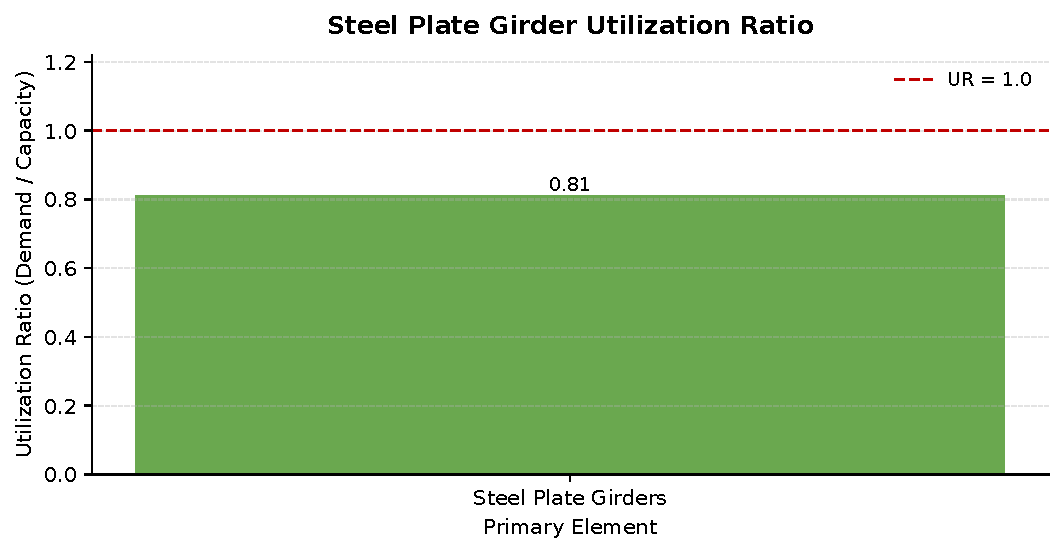
\includegraphics[width=0.82\textwidth]{assets/ur_steel_plate_girders.pdf}
\vspace{0.5em}
\caption{\small Steel Plate Girder Utilization Ratio}
\vspace{-0.5em}
\end{figure}
\vspace{0.5em}
\begin{figure}[H]
\vspace{-0.5em}
\centering
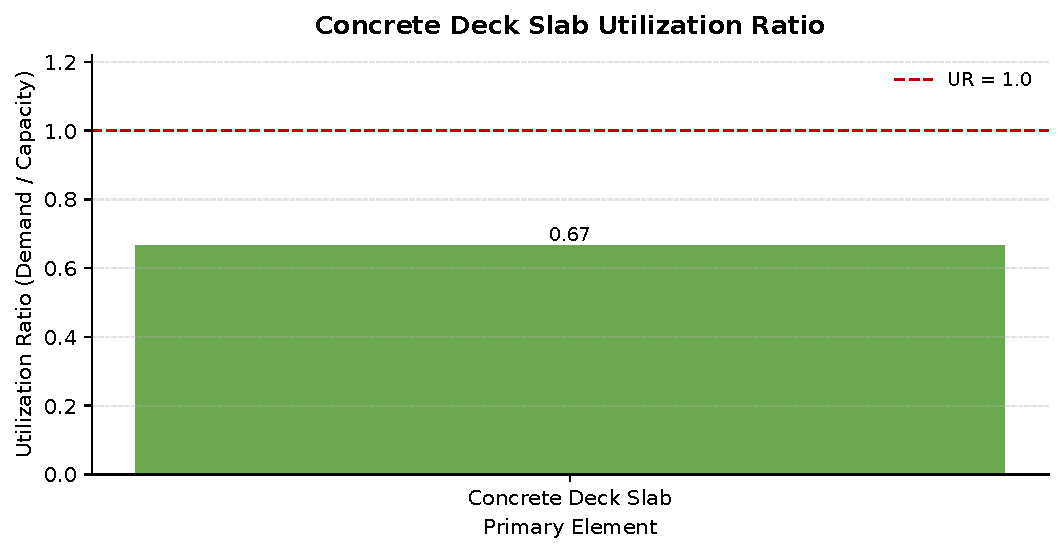
\includegraphics[width=0.82\textwidth]{assets/ur_concrete_deck_slab.pdf}
\vspace{0.5em}
\caption{\small Concrete Deck Slab Utilization Ratio}
\vspace{-0.5em}
\end{figure}
\vspace{0.5em}
\begin{figure}[H]
\vspace{-0.5em}
\centering
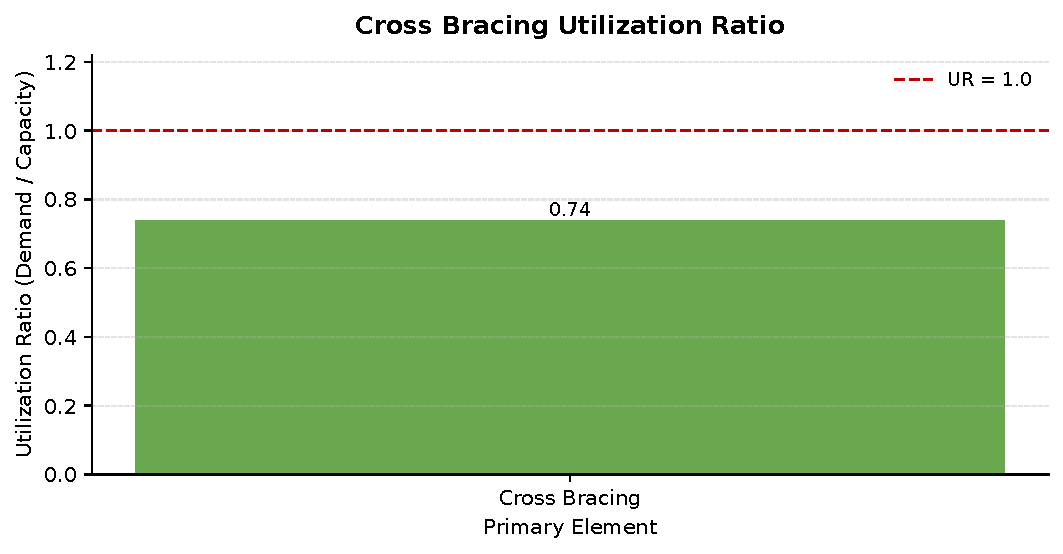
\includegraphics[width=0.82\textwidth]{assets/ur_cross_bracing.pdf}
\vspace{0.5em}
\caption{\small Cross Bracing Utilization Ratio}
\vspace{-0.5em}
\end{figure}
\vspace{0.5em}
\begin{figure}[H]
\vspace{-0.5em}
\centering
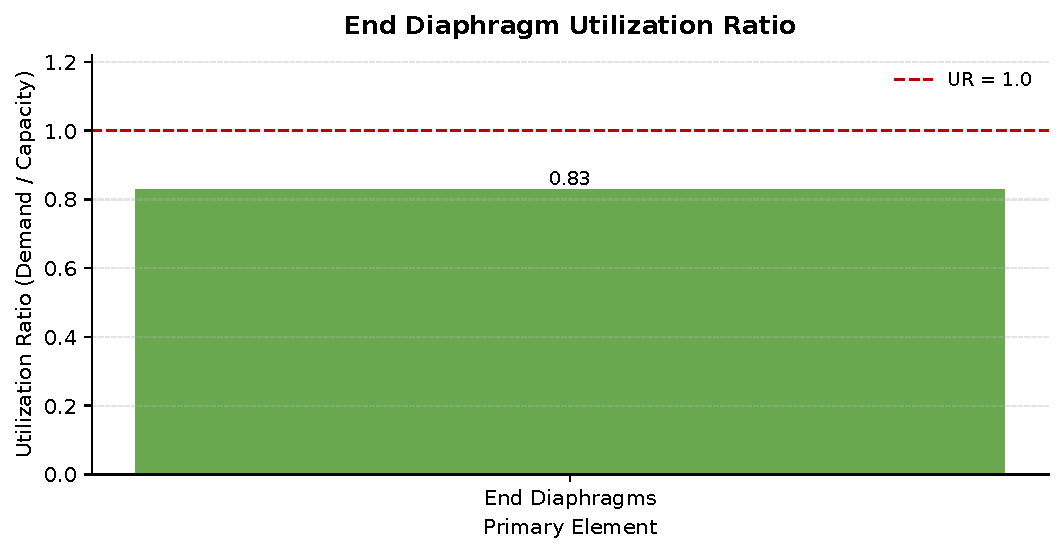
\includegraphics[width=0.82\textwidth]{assets/ur_end_diaphragms.pdf}
\vspace{0.5em}
\caption{\small End Diaphragm Utilization Ratio}
\vspace{-0.5em}
\end{figure}



\chapter{Drawings and Visualizations}
\label{ch:drawings}

This section presents CAD-generated views of the designed bridge and its components. All views are generated automatically by OsdagBridge using pythonOCC.

\section{Bridge Configuration and Layout}
\label{sec:bridge-layout}

\begin{figure}[H]
\centering
\fbox{\parbox{0.97\textwidth}{
\textit{[ PLACEHOLDER:  Overall 3D Bridge Superstructure ]}
}}
\caption{Overall 3D Bridge Superstructure}
\label{fig:bridge-3d}
\end{figure}


\begin{figure}[H]
\centering
\fbox{\parbox{0.97\textwidth}{
\textit{[ PLACEHOLDER:  Typical Cross Section ]}
}}
\caption{Typical Cross Section}
\label{fig:cross-section}
\end{figure}


\begin{figure}[H]
\centering
\fbox{\parbox{0.97\textwidth}{
\textit{[ PLACEHOLDER:  Top View ]}
}}
\caption{Top View}
\label{fig:top-view}
\end{figure}


\section{Plate Girder --- Detailed Views}
\label{sec:girder-views}

\begin{figure}[H]
\centering
\fbox{\parbox{0.97\textwidth}{
\textit{[ PLACEHOLDER:  3D View of Plate Girders ]}
}}
\caption{3D View of Plate Girders}
\label{fig:girder-3d}
\end{figure}


\begin{figure}[H]
\centering
\fbox{\parbox{0.97\textwidth}{
\textit{[ PLACEHOLDER:  Cross Section of Plate Girder ]}
}}
\caption{Cross Section of Plate Girder}
\label{fig:girder-xsec}
\end{figure}


\begin{figure}[H]
\centering
\fbox{\parbox{0.97\textwidth}{
\textit{[ PLACEHOLDER:  Side View of Girder ]}
}}
\caption{Side View of Girder}
\label{fig:girder-side}
\end{figure}


\section{Cross Bracing Detail}
\label{sec:bracing-detail}

\begin{figure}[H]
\centering
\fbox{\parbox{0.97\textwidth}{
\textit{[ PLACEHOLDER:  Cross Bracing Layout ]}
}}
\caption{Cross Bracing Layout}
\label{fig:cb-layout}
\end{figure}


\noindent
\begin{minipage}[t]{0.31\textwidth}
\centering
\fbox{\parbox{0.95\linewidth}{\centering\textit{[ Cross Bracing -- Bracing Section ]}}}
\captionof{figure}{Cross Bracing -- Bracing Section}
\label{fig:cb-bracing-sec}
\end{minipage}
\hfill
\begin{minipage}[t]{0.31\textwidth}
\centering
\fbox{\parbox{0.95\linewidth}{\centering\textit{[ Cross Bracing -- Top Chord Section ]}}}
\captionof{figure}{Cross Bracing -- Top Chord Section}
\label{fig:cb-top-chord}
\end{minipage}
\hfill
\begin{minipage}[t]{0.31\textwidth}
\centering
\fbox{\parbox{0.95\linewidth}{\centering\textit{[ Cross Bracing -- Bottom Chord Section ]}}}
\captionof{figure}{Cross Bracing -- Bottom Chord Section}
\label{fig:cb-bottom-chord}
\end{minipage}
            

\section{End Diaphragm Detail}
\label{sec:diaphragm-detail}

\begin{figure}[H]
\centering
\fbox{\parbox{0.97\textwidth}{
\textit{[ PLACEHOLDER:  End Diaphragm Layout ]}
}}
\caption{End Diaphragm Layout}
\label{fig:ed-layout}
\end{figure}


\noindent
\begin{minipage}[t]{0.31\textwidth}
\centering
\fbox{\parbox{0.95\linewidth}{\centering\textit{[ End Diaphragm -- Bracing Section ]}}}
\captionof{figure}{End Diaphragm -- Bracing Section}
\label{fig:ed-bracing-sec}
\end{minipage}
\hfill
\begin{minipage}[t]{0.31\textwidth}
\centering
\fbox{\parbox{0.95\linewidth}{\centering\textit{[ End Diaphragm -- Top Chord Section ]}}}
\captionof{figure}{End Diaphragm -- Top Chord Section}
\label{fig:ed-top-chord}
\end{minipage}
\hfill
\begin{minipage}[t]{0.31\textwidth}
\centering
\fbox{\parbox{0.95\linewidth}{\centering\textit{[ End Diaphragm -- Bottom Chord Section ]}}}
\captionof{figure}{End Diaphragm -- Bottom Chord Section}
\label{fig:ed-bottom-chord}
\end{minipage}



\chapter{Bill of Materials}
\label{ch:material-takeoff}
\begin{longtable}{|C{0.84cm}|L{3.19cm}|C{2.1cm}|C{1.76cm}|C{1.51cm}|C{1.43cm}|C{1.51cm}|}
\captionsetup{justification=centering,font={small,it}}
\caption{Bill of Materials for Superstructure}\\
\hline
\textbf{\parbox[t][1.75cm][c]{\linewidth}{\centering S.N.}} & \textbf{\parbox[t][1.75cm][c]{\linewidth}{\centering Item\\Description}} & \textbf{\parbox[t][1.75cm][c]{\linewidth}{\centering Volume}} & \textbf{\parbox[t][1.75cm][c]{\linewidth}{\centering Quantity}} & \textbf{\parbox[t][1.75cm][c]{\linewidth}{\centering Total\\Volume\\(m$^3$)}} & \textbf{\parbox[t][1.75cm][c]{\linewidth}{\centering Weight\\(t)}} & \textbf{\parbox[t][1.75cm][c]{\linewidth}{\centering Total\\Weight\\(t)}} \\
\hline
\endfirsthead
\hline
\textbf{\parbox[t][1.75cm][c]{\linewidth}{\centering S.N.}} & \textbf{\parbox[t][1.75cm][c]{\linewidth}{\centering Item\\Description}} & \textbf{\parbox[t][1.75cm][c]{\linewidth}{\centering Volume}} & \textbf{\parbox[t][1.75cm][c]{\linewidth}{\centering Quantity}} & \textbf{\parbox[t][1.75cm][c]{\linewidth}{\centering Total\\Volume\\(m$^3$)}} & \textbf{\parbox[t][1.75cm][c]{\linewidth}{\centering Weight\\(t)}} & \textbf{\parbox[t][1.75cm][c]{\linewidth}{\centering Total\\Weight\\(t)}} \\
\hline
\endhead
1 & Structural Steel (IS 2062) for Girders & $0.03\text{ m}^2 \allowbreak{}\times\allowbreak{} 30.00\text{ m} = 0.75\text{ m}^3$ & 4 & 3.00 & 5.89 & 23.55 \\
\hline
2(a) & Cross Bracing - Top Chord & N.A. & N.A. & N.A. & N.A. & N.A. \\
\hline
2(b) & Cross Bracing - Bottom Chord & N.A. & N.A. & N.A. & N.A. & N.A. \\
\hline
2(c) & Cross Bracing - Diagonal Chord & N.A. & N.A. & N.A. & N.A. & N.A. \\
\hline
2(d) & End Diaphragms & N.A. & N.A. & N.A. & N.A. & N.A. \\
\hline
3(a) & Stiffeners - Bearing & N.A. & N.A. & N.A. & N.A. & N.A. \\
\hline
3(b) & Stiffeners - Intermediate & N.A. & N.A. & N.A. & N.A. & N.A. \\
\hline
4 & Connections & $10\% \allowbreak{}\times\allowbreak{} 3.00\text{ m}^3 = 0.30\text{ m}^3$ & 1 & 0.30 & 2.35 & 2.35 \\
\hline
5 & Concrete (M40) for Deck Slab & $10.00\text{ m} \allowbreak{}\times\allowbreak{} 0.25\text{ m} \allowbreak{}\times\allowbreak{} 30.00\text{ m} = 75.00\text{ m}^3$ & 1 & 75.00 & 187.50 & 187.50 \\
\hline
6 & Reinforcement Steel (Fe 500) & $0.04\text{ m}^2 \allowbreak{}\times\allowbreak{} 30.00\text{ m} = 1.15\text{ m}^3$ & 1 & 1.15 & 9.00 & 9.00 \\
\hline
7 & Shear Stud Connectors & N.A. & N.A. & N.A. & N.A. & N.A. \\
\hline
8 & Crash Barrier & N.A. & N.A. & N.A. & N.A. & N.A. \\
\hline
\end{longtable}
\vspace{1em}
\begin{figure}[H]
\vspace{-0.5em}
\centering
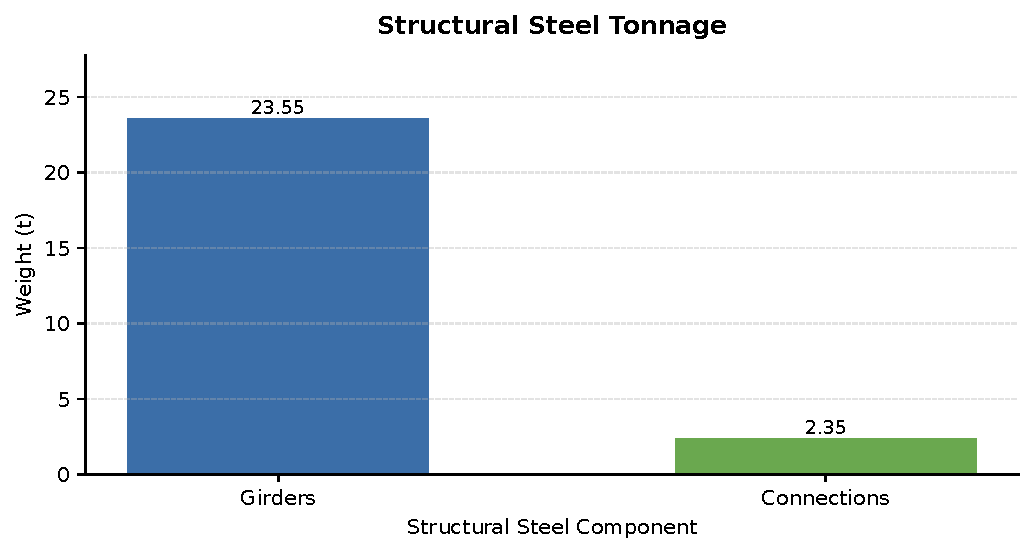
\includegraphics[width=0.82\textwidth]{assets/material_steel_quantities.pdf}
\vspace{0.5em}
\caption{\small Structural Steel Tonnage Summary}
\vspace{-0.5em}
\end{figure}
\vspace{0.5em}
\begin{figure}[H]
\vspace{-0.5em}
\centering
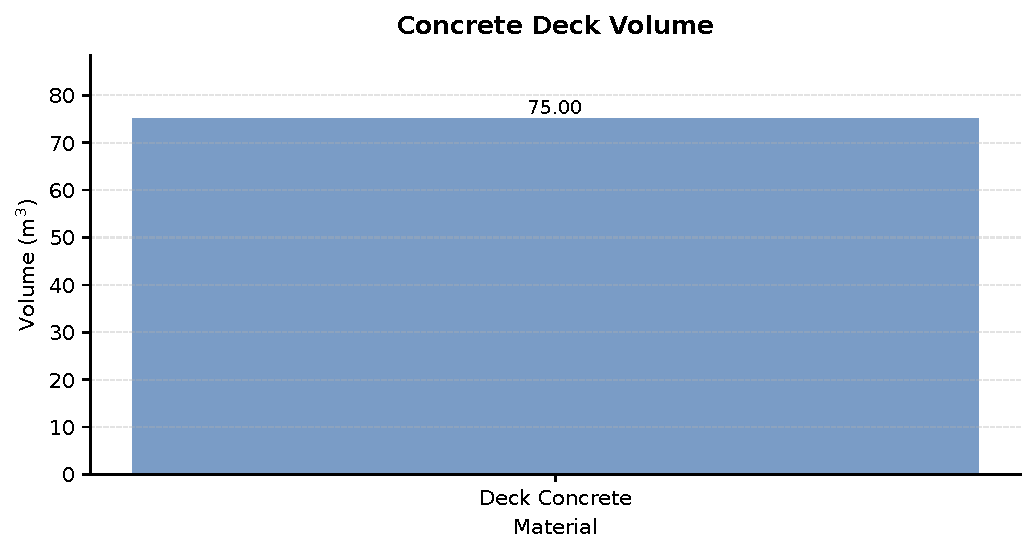
\includegraphics[width=0.82\textwidth]{assets/material_concrete_quantity.pdf}
\vspace{0.5em}
\caption{\small Concrete Deck Volume Summary}
\vspace{-0.5em}
\end{figure}
\vspace{0.5em}
\begin{figure}[H]
\vspace{-0.5em}
\centering
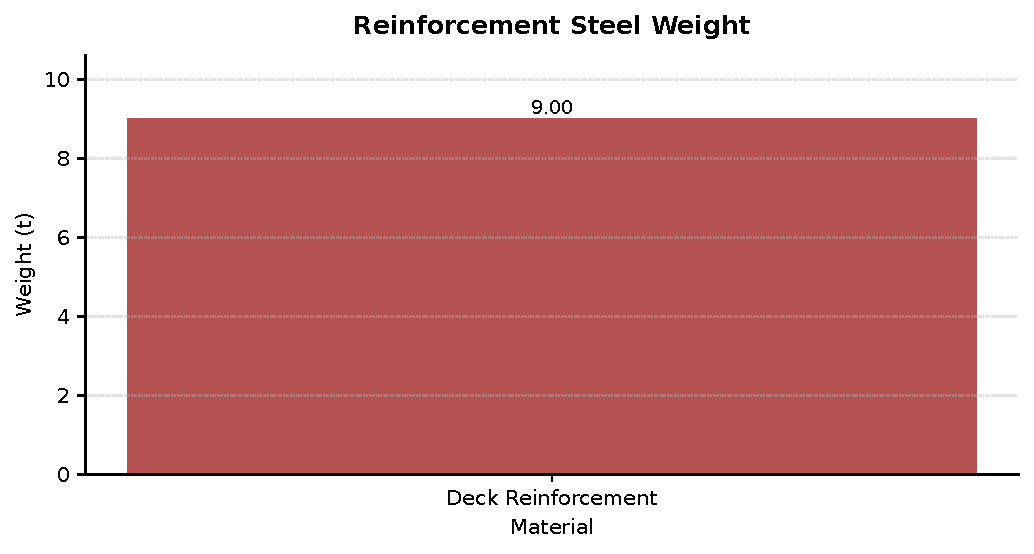
\includegraphics[width=0.82\textwidth]{assets/material_reinforcement_quantity.pdf}
\vspace{0.5em}
\caption{\small Deck Reinforcement Steel Summary}
\vspace{-0.5em}
\end{figure}

\chapter{Standards \& Assumptions}
\label{ch:Design Standards}

This section provides references to standards used to calibrate the OsdagBridge
design modules, and notes the limitations of the current software version.

\section{Design Standards}
\label{sec:design_standards}

The following Indian Road Congress (IRC) codes and Indian Standards (IS) 
form the basis of all design calculations in this software.

\vspace{0.5cm}

\begin{table}[H]
\centering
\captionsetup{justification=centering,font={small,it}}
\caption{IRC Codes}
\begin{tabular}{|C{2.01cm}|C{1.28cm}|L{10.85cm}|}
\hline
\textbf{Code} & \textbf{Year} & \textbf{Title / Scope} \\
\hline
IRC 5 & 2015 & General Features of Design - carriageway widths, kerb, footpath dimensions \\
\hline
IRC 6 & 2017 & Loads and Load Combinations - dead load, live load, impact, wind, temperature, etc. \\
\hline
IRC 22 & 2015 & Composite Construction (LS) - Composite section properties, ULS/SLS design, shear connectors \\
\hline
IRC 24 & 2010 & Steel Road Bridges (LS) - Stiffener design, skew angle limits, diaphragm requirements \\
\hline
IRC 112 & 2020 & Concrete Road Bridges - Deck slab flexure, shear, crack width, reinforcement \\
\hline
IRC SP 114 & 2018 & Seismic Design of Road Bridges \\
\hline
\end{tabular}
\end{table}

\begin{table}[H]
\centering
\captionsetup{justification=centering,font={small,it}}
\caption{IS Codes}
\begin{tabular}{|C{2.55cm}|C{1.28cm}|L{10.3cm}|}
\hline
\textbf{Code} & \textbf{Year} & \textbf{Scope} \\
\hline
IS 800 & 2007 & Steel construction - tension, compression, bending, shear, LTB, stiffeners, combined checks \\
\hline
IS 456 & 2000 & Concrete - simplified stress-block for deck moment capacity \\
\hline
IS 1786 & 2008 & Reinforcement steel properties \\
\hline
IS 1893 (Part 3) & 2014 & Earthquake resistant design \\
\hline
IS 2062 & 2011 & Structural steel - yield and ultimate strength by grade \\
\hline
\end{tabular}
\end{table}

\clearpage
\section{Analysis and Design Assumptions of This Version}
\label{sec:analysis_design_assumptions}

\textbf{Structural Analysis}

\begin{itemize}
    \item All girders are modelled as simply supported; continuous spans are not currently supported.
    \item A 3D grillage model (OSPGrillage) is used for load distribution. Grillage members carry composite section properties after the construction stage.
    \item The transverse member forces are computed using an approximate 2D frame analogy. For irregular or skewed geometries, a 3D FEM is recommended.
    \item Fixed bearing stiffness is modelled as $k = 1{,}000{,}000 \,\text{kN/m}$ (virtually rigid); free/expansion bearing as $k = 100 \, \text{kN/m}$.
    \item Construction stage sequence analysis is approximate. Detailed staged analysis should be performed for long-term deflection checks.
\end{itemize}

\textbf{Composite Action}

\begin{itemize}
    \item Full shear connection is assumed at ULS with headed stud connectors designed per IRC 22:2015 Cl.606.
    \item Short-term composite section properties (modular ratio $n = E_s/E_{cm}$) are used for ULS checks.
    \item Long-term composite section properties (with creep-adjusted modular ratio) are used for SLS deflection and crack-width checks.
    \item Pre-composite stage: the steel girder alone resists all construction loads prior to concrete gaining strength.
\end{itemize}


\textbf{Material Properties (IRC 22:2015 Annex III)}

\begin{itemize}
\item Steel: $E_s = 200{,}000 \, \text{MPa}, \ G_s = 80{,}000 \, \text{MPa}, \ \nu = 0.30, \ \alpha = 11.7 \times 10^{-6}/^\circ\mathrm{C}$ (grade-independent).
\item Minimum structural concrete grade: M25.
\item Default reinforcement grade: Fe500.
\end{itemize}

\textbf{Partial Safety Factors (IRC 22:2015 Cl.601.4)}

\begin{itemize}
\item $\gamma_{m0}$ (steel yield, ULS) = 1.10
\item $\gamma_{m1}$ (steel ultimate, ULS) = 1.25
\item Reinforcement (ULS) = 1.15
\item Welds -- shop: 1.25; field: 1.50
\item Fatigue ($\gamma_{mft}$) = 1.35
\end{itemize}

\textbf{Loading}

\begin{itemize}
\item Dead load densities per IRC 6:2017 Cl.203: structural steel $78.5 \ \text{kN/m}^3$, concrete $25.0 \ \text{kN/m}^3$, bituminous wearing course $24.0 \ \text{kN/m}^3$.
\item Multi-lane live load reduction factors per IRC 6:2017 Cl.204.4 Table 6A: 1st lane = 1.0, 2nd lane = 0.8, 3rd lane onwards = 0.4.
\item Impact factor (dynamic load allowance) computed from span per IRC 6:2017 Cl.208.2/208.3.
\item Wind load applied as transverse, longitudinal, and vertical components per IRC 6:2017 Cl.209.3.3--209.3.5.
\end{itemize}

\textbf{Serviceability Limits}

\begin{itemize}
\item Deflection limits (IRC 22:2015 Cl.604.3.2): live load + impact $\leq L/800$; total $\leq L/600$.
\item SLS stress limits: concrete $\sigma_c \leq 0.48 f_{ck}$; rebar $\sigma_s \leq 0.80 f_{yk}$; steel $f_e \leq 0.9 f_y$.
\item Permissible crack width: $w_k \leq 0.3 \ \text{mm}$ (bridge deck, exposure class XS2/XD2 per IRC 112:2020 Cl.12.3.2).
\end{itemize}

\textbf{Fatigue}

\begin{itemize}
\item Reference fatigue life: $N_{sc} = 2 \times 10^6$ cycles (IRC 22:2015 Cl.605).
\item Constant stress range is assumed. A thickness correction factor $\mu_r$ is applied for plate thickness $> 25 \ \text{mm}$.
\end{itemize}

\textbf{Stiffener Design}

\begin{itemize}
\item Intermediate transverse stiffener and bearing stiffener design follows IS 800:2007 Cl.8.7.2/8.7.3 and IRC 24:2010 Cl.509.7.2/509.7.3.
\end{itemize}


\section{Known Limitations of This Version}
\label{sec:limitations}

\begin{itemize}
\item Substructure (piers, pile caps, foundations) and bearing design are not included.
\item Splice connection design is not implemented.
\item Skew angle $>$ 15 degrees requires independent manual analysis (IRC 24 Cl. 504.8).
\item Construction stage sequence analysis is approximate; detailed staged analysis
  should be performed for long-term deflection checks.
\item The grillage analysis assumes simply supported boundary conditions;
  continuous spans are not currently supported.
\end{itemize}


\chapter*{References}
\addcontentsline{toc}{chapter}{References}


\begin{enumerate}

\item IRC 5 (2024) --- \textit{Standard Specifications and Code of Practice for Road Bridges, Section I: General Features of Design.}

\item IRC 6 (2017) --- \textit{Standard Specifications and Code of Practice for Road Bridges, Section II: Loads and Load Combinations.}

\item IRC 22 (2014) --- \textit{Standard Specifications and Code of Practice for Road Bridges, Section VI: Composite Construction (Limit State Design).}

\item IRC 24 (2010) --- \textit{Standard Specifications and Code of Practice for Road Bridges, Section V: Steel Road Bridges (Limit State Method).}

\item IRC 112 (2011) --- \textit{Code of Practice for Concrete Road Bridges.}

\item IRC SP 114 (2018) --- \textit{Guidelines for Seismic Design of Road Bridges.}

\item IS 800 (2007) --- \textit{Indian Standard: General Construction in Steel --- Code of Practice.}

\item IS 2062 (2011) --- \textit{Hot Rolled Medium and High Tensile Structural Steel --- Specification.}

\item Subramanian, N. (2008). \textit{Design of Steel Structures.} Oxford University Press.

\item Steel-INSDAG Teaching Resource Materials. \url{https://www.steel-insdag.org}

\end{enumerate}

\end{document}